\section{Experiments}

We conduct automatic evaluations on both MS-COCO and Localized Narratives to compare with previous work. On MS-COCO and \bcp, we also obtain human side-by-side evaluations for \bdraw 20B to compare with a strong retrieval baseline, as well as the XMC-GAN model \cite{zhang2021cross}, which has the best FID out of all publicly available models at the time of writing. We also conduct human evaluation on two \bdraw models with parameters 3B and 20B on \bcp, and provide a detailed breakdown on categories. By default, \bdraw samples 16 images per text prompt and uses a CoCa model to rank the outputs (see Section~\ref{secs:sampling_cf_coca}).

\subsection{Retrieval Baseline}  \label{secs:retrieval_model}
Perhaps the most compelling use for text-to-image generation models is creating novel images for situations that have never been depicted. Strong models should thus be more effective than an approach that simply retrieves candidate images from a large dataset. We implement a retrieval baseline as follows. For every training data example, we compute image embeddings from an EfficientNet-L2 ALIGN-based model~\cite{jia2021scaling}. Then, given a text prompt, we identify the nearest training image measured by the alignment between the text prompt embedding from the ALIGN-based model and the image embeddings. This can be done at the scale of our data by using efficient similarity search libraries such as ScaNN~\cite{avq_2020}. These retrieved examples (from the training set) are then provided as the output of the baseline, to be evaluated by images actually generated by our models. We manually visualize the retrieved images given the text prompts and observe that this retrieval approach represents a high-quality baseline, especially for common text descriptions.

To compare with \bdraw generated images, we report retrieval baseline results under two settings that we characterize as \textit{zero-shot} and \textit{finetuned} to align with the model evaluation terminology. For MS-COCO, retrieval over our training data is ``zero-shot'', while retrieval over MS-COCO's train split is ``finetuned'' -- corresponding to out-of-dataset and in-dataset retrieval, respectively. We compare \bdraw generated images with retrieved images using both automated measures and human evaluation for both image realism and image-text alignment.

\subsection{Evaluation Metrics}

We evaluate using two primary axes: (1) generated image quality, and (2) alignment of the generated image with the input text. We report both automated quantitative metrics and human evaluation results. In addition, we show example model outputs for qualitative assessment and comparison.

\textbf{Automatic image quality.} Similar to prior work in text-to-image generation, we use the Fr\'echet Inception Distance (FID)~\cite{heusel2017gans} as the primary automated metric for measuring image quality.\footnote{We use \url{https://github.com/mseitzer/pytorch-fid} for computing FID scores.} FID is computed by running generated and real images through the Inception v3~\cite{szegedy2016rethinking} model, and extracting features from the last pooling layer of the model. The Inception features of the generated and real images are used to fit two separate multi-variate Gaussians. Finally, the FID score is computed by measuring the Fr\'echet distance between the two multivariate Gaussian distributions. Following \cite{Xu18,zhang2021cross,ramesh2021zero}, we use 30,000 generated and real image samples for evaluation on MS-COCO (2014) using the same DALL-E input preprocessing (Section B.2. Training in~\cite{ramesh2021zero}) with \(256{\times}256\) image resolution. The validation set of the Localized Narratives COCO split contains only 5,000 unique images, so we follow ~\cite{zhang2021cross} in oversampling the captions to acquire 30,000 generated images.

\textbf{Automatic image-text alignment.} Following DALL-Eval~\cite{Cho2022DallEval}, we also measure text-image fit through automated captioning evaluation (or captioner evaluation): an image output by the model is captioned with a pretrained VL-T5 model~\cite{cho2021vlt5} and then the similarity of the input prompt and and the generated caption is assessed via BLEU~\cite{Papineni2002}, CIDEr~\cite{Vedantam2015}, METEOR~\cite{denkowski2014} and SPICE~\cite{spice2016}.  

\textbf{Human side-by-side.} We follow previous work \cite{zhang2021cross, ramesh2021zero} in doing side-by-side evaluations in which human annotators are presented with two outputs for the same prompt and are asked to choose which output is a higher quality image (generally, better with respect to image realism) and which is a better match to the input prompt (image-text alignment). The models are anonymized and the pairs are randomly ordered (left \vs\ right) for each presentation to an annotator, and each pair is judged by five independent annotators. We graphically show the gradual breakdown of results for each model in terms of the number of examples where it obtains 0, 1, 2, 3, 4 or 5 votes. In addition, we highlight the percentage of examples where each model has obtain the majority (three or more votes), as a summary of the comparison. See Appendix~\ref{secs:appendix_human_eval} for a screenshot of our annotator interface.

\subsection{Main Results} \label{secs:main_results}

\begin{table*}[t]
\begin{center}
\scriptsize
\setlength\tabcolsep{2pt}
\resizebox{\textwidth}{!}{
\begin{tabular}{lcccccc@{\hspace{4mm}}cc}
\multicolumn{1}{l}{\multirow{2}{*}{\textbf{Approach}}} && \multicolumn{1}{c}{\multirow{2}{*}{\textbf{Model Type}}} && \multicolumn{2}{c}{\textbf{MS-COCO FID ($\downarrow$)}} && \multicolumn{2}{c}{\textbf{LN-COCO FID ($\downarrow$)}} \\
\cmidrule{5-6} \cmidrule{8-9}
& && & Zero-shot & Finetuned & & Zero-shot & Finetuned  \\
\toprule
Random Train Images~\cite{gafni2022make}  && - && \multicolumn{2}{c}{2.47} && \multicolumn{2}{c}{-} \\
Retrieval Baseline  && -   &&  17.97 & \pz6.82  && 33.59 & 16.48   \\
\midrule
TReCS~\cite{trecs2020}  && GAN & & - & - &  & - & 48.70  \\
XMC-GAN~\cite{zhang2021cross}  && GAN & & - & \pz9.33 &  & - & 14.12  \\
DALL-E~\cite{ramesh2021zero}  && Autoregressive  & & $\sim$28\pzz\pzz & - &  & - & -   \\
CogView~\cite{ding2021cogview}  && Autoregressive & & 27.1\pz & - & & - & -    \\
CogView2~\cite{cogview2}  && Autoregressive & & 24.0\pz & 17.7\pz & & - & -    \\
GLIDE~\cite{nichol2021glide}  && Diffusion & & 12.24 & - &  & - & -     \\
Make-A-Scene~\cite{gafni2022make}  && Autoregressive & & 11.84 & \pz7.55 &  & - & -     \\
DALL-E 2~\cite{ramesh2022hierarchical}  && Diffusion & & 10.39 & - &  & - & -   \\
Imagen~\cite{imagen}  && Diffusion & & \pz\textbf{7.27} & - &  & - & -   \\
\midrule
\bdraw  &&  Autoregressive  && \pz\textbf{\fid} & \pz\textbf{\fidft} && \textbf{15.97} & \pz\textbf{8.39} \\
\bottomrule
\end{tabular}
}
\caption{Comparison with previous work on the MS-COCO (2014)~\cite{lin2014microsoft} and Localized Narratives (COCO split)~\cite{PontTuset_eccv2020} validation sets. When available, we report results for both zero-shot and finetuned models. Retrieval models either perform retrieval over our training set (``zero-shot''), or the respective MS-COCO and LN-COCO training sets (``finetuned''). \bdraw samples 16 images per text prompt and uses a CoCa model to rank the outputs (Section~\ref{secs:sampling_cf_coca}). Similar to DALL-E 2~\cite{ramesh2022hierarchical}, we use guidance scale 1.2 for all above results. We report zero-shot FID score of other model sizes in Figure~\ref{tabs:scaling_results}.
}
\label{table:coco_results}
\end{center}
\vspace{-0.2in}
\end{table*}

Table~\ref{table:coco_results} presents our main results of automated image quality evaluation. \bdraw achieves a comparable zero-shot FID score 7.23 compared with diffusion-based model Imagen~\cite{imagen}. When finetuned, \bdraw achieves state-of-the-art FID score of 3.22, a dramatic improvement over previous best finetuned FID 7.55 from an autoregressive model, Make-a-Scene~\cite{gafni2022make}. It is also better than the in-dataset retrieval baseline, with an FID score 6.82. We note that the retrieval baseline is worse than using 30,000 random samples from MS-COCO real training set images -- which obtains an FID of 2.47. The root cause is that the retrieval model often selects the same images for similar types of prompts, leading to duplicates in the retrieved images for evaluation. For example, there are only 17,782 unique retrieved MS-COCO train images for 30,000 validation text prompts, leading to worse diversity and poorer FID score as compared to the 30,000 random samples from the train set. We also show qualitative comparisons (Appendix~\ref{secs:appendix_qualitative_comparison}, Figure~\ref{figs:coco_model_comparison}) of non-cherry-picked \bdraw sampled images along with outputs of other approaches~\cite{ramesh2021zero, nichol2021glide, gafni2022make, ramesh2022hierarchical} on MS-COCO prompts. \bdraw demonstrates strong generalization without finetuning on specific domains like MS-COCO, and it achieves a high degree of image realism -- often very close to that of real images.

For LN-COCO, \bdraw achieves a finetuned FID score of 8.29, which is a massive improvement over XMC-GAN's finetuned result of 14.12 and the retrieval baseline's 16.48. Moreover, \bdraw achieves a zero-shot FID score of 15.97, which nearly matches XMC-GAN's finetuned score (trained on LN-COCO set). We visualize and compare side-by-side with XMC-GAN and find the zero-shot images produced by \bdraw are qualitatively much better in realism and image-text fit compared to images produced by XMC-GAN, which we offer as a cautionary tale that researchers should not rely solely on FID for comparison of text-to-image generation models. 

\subsection{More Results on MS-COCO} \label{secs:more_results}

\textbf{Automatic image-text alignment evaluation.}
Table~\ref{tabs:image-text-auto} provides results of \bdraw on the captioner evaluation~\cite{Cho2022DallEval} as an automatic image-text alignment measure. \bdraw outperforms other models on this measure, and it closes much of the gap to the scores obtained for captions generated from the ground truth images. The retrieval baseline performs comparable to \bdraw. Unlike FID scores, random train images perform considerably worse on the captioner evaluation, as expected. The captioner evaluation complements FID score evaluation as an automatic image-text alignment measurement for text-to-image generation models; however, we also note these results are limited by the captioner model's~\cite{cho2021vlt5} ability to discriminate between outputs from different approaches.

\begin{table}
\begin{center}
\begin{tabular}{@{}lcccc@{}}
Approach & BLEU ($\uparrow$) & METEOR ($\uparrow$) & CIDEr ($\uparrow$) & SPICE ($\uparrow$) \\
\toprule
Random Train Images & \pz4.4 & \pz9.2 & \pz4.8 & \pz2.0 \\
Retrieval Baseline & 24.7 & 23.9 & 84.1 & 16.6 \\
Ground Truth (upper bound) & 32.5 & 27.5 & 108.3\pz & 20.4 \\
\midrule
DALL-E\textsuperscript{Small}\footnotemark[5]     & \pz9.3  & 12.9 & 20.2  & \pz5.6 \\
ruDALL-E-XL\footnotemark[6]    & 13.9 & 16.0 & 38.7  & \pz8.7  \\
minDALL-E \cite{mindalle}       & 16.6 & 17.6 & 48.0  & 10.5 \\
X-LXMERT \cite{Cho2020XLXMERTPC}        & 18.5 & 19.1 & 55.8  & 12.1 \\
\midrule
\bdraw & \textbf{26.4} & \textbf{23.9} & \textbf{83.9} & \textbf{16.5} \\
\bottomrule
\end{tabular}
\vspace{0.1in}
\caption{Comparison with prior work on captioner evaluation on the MS-COCO 5K test set \cite{Karpathy2017DeepVA} with baselines from DALL-Eval~\cite{Cho2022DallEval}. Ground Truth represents the theoretical upper bound on this evaluation with captions generated using MS-COCO images as inputs to the VL-T5 model~\cite{cho2021vlt5}. \bdraw samples 16 images per text prompt and uses a CoCa~\cite{yu2022coca} model to rank the outputs (Section~\ref{secs:sampling_cf_coca}). \label{tabs:image-text-auto}}
\vspace{-0.2in}
\end{center}
\end{table}

\footnotetext[5]{\url{https://github.com/lucidrains/DALLE-pytorch}}
\addtocounter{footnote}{1}
\footnotetext[6]{\url{https://rudalle.ru}}
\addtocounter{footnote}{1} %


\begin{figure}[tbh!]
    \centering
    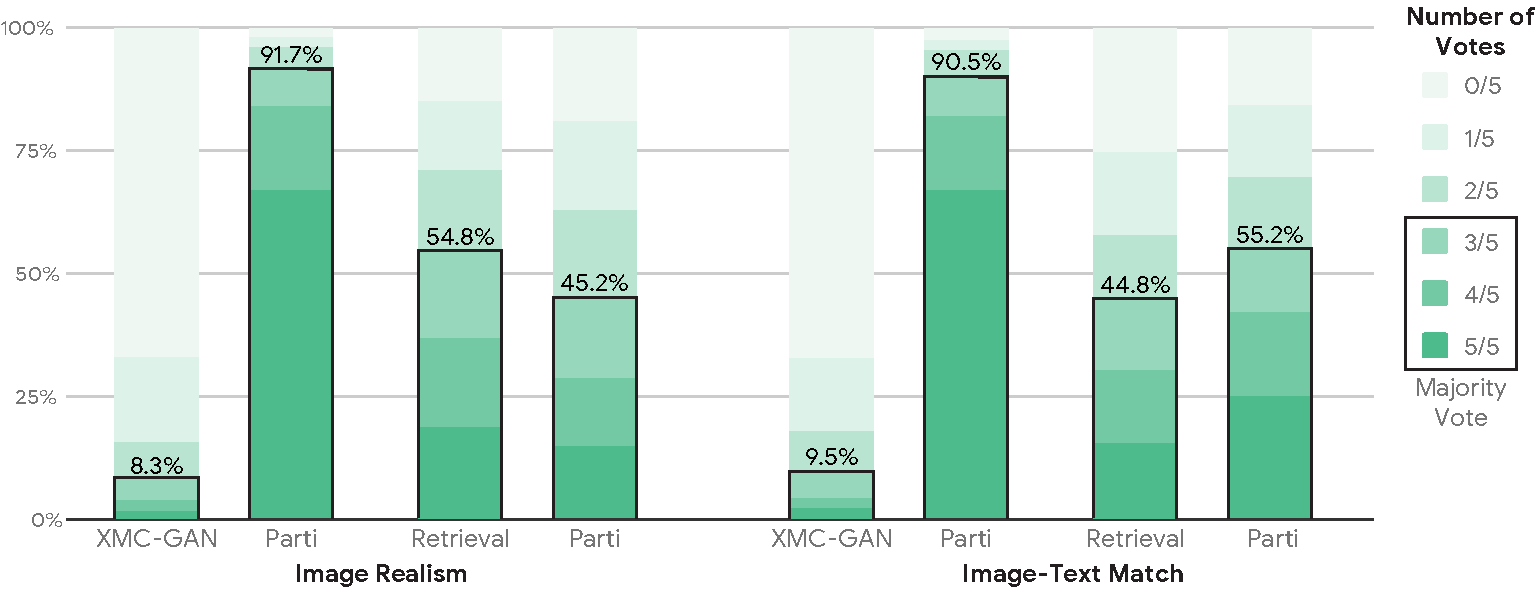
\includegraphics[width=1.0\textwidth]{figures/human_evals_coco.pdf}
    \caption{Human evaluation results over 1,000 randomly sampled prompts from the MS-COCO (2014) validation set. Each prompt is rated by 5 independent human evaluators. The zero-shot \bdraw models are used in all comparisons. Our model significantly outperforms XMC-GAN~\cite{zhang2021cross}, despite the latter being finetuned on MS-COCO. When compared against the retrieval model (retrieval over about 4B training images), \bdraw is better on image-text match, but worse on image realism (as retrieved images are real images).}
    \label{fig:human_evals_coco}
\end{figure}

\textbf{Human evaluations.} For MS-COCO, we compare our \textit{zero-shot} generation results against the \textit{finetuned} XMC-GAN~\cite{zhang2021cross} model, which has best the FID out of all publicly available models with available images of the same MS-COCO prompts, at the time of writing. For each prompt, the output from \bdraw and XMC-GAN are anonymized and shown to 1,000 independent human evaluators. The results are summarized and shown in Figure~\ref{fig:human_evals_coco}.  Even though \bdraw is not trained on MS-COCO captions or images, our results are overwhelmingly preferred by human annotators over XMC-GAN outputs: 91.7\% preference score for image realism and 90.5\% for image-text match.\footnote{We analyzed the cases in which XMC-GAN is rated as more realistic compared to \bdraw, and found that most of these examples were due to \bdraw producing illustrations or cartoons, rather than photo-realistic images. While these were generally well aligned with the given prompts, the evaluation likely disadvantages \bdraw since MS-COCO is entirely focused on photographs and descriptions of them.}
When compared against the retrieval model on MS-COCO, \bdraw is evaluated as slightly worse on image realism (45.2\% compared to 54.8\%)
but evaluated as better on image-text match (55.2\% compared to 44.8\%). This shows that in nearly half of the comparisons between \bdraw's output and \textit{real} images, the former \textit{generated} images were judged as more realistic by people---a strong statement of the visual quality of images produced by the model. The fact that \bdraw outputs are preferred for image-text match shows that generation is an important means of producing accurate visual depictions of even the mostly quotidian scenes described in MS-COCO captions.

\begin{figure}[tbh!]
\centering
\resizebox{0.28\textwidth}{!}{
\begin{tabular}[b]{lc}
\toprule
\multicolumn{2}{c}{\textbf{MS-COCO (zero-shot)}} \\
\textbf{Parameters} & \textbf{FID $\downarrow$} \\
\toprule
 350M & 14.10 \\
 750M & 10.71 \\
 \pzz3B  & \pz8.10 \\
 \pz20B  & \pz\fid \\
\bottomrule
\vspace{0.15in}
\end{tabular}
}
\qquad
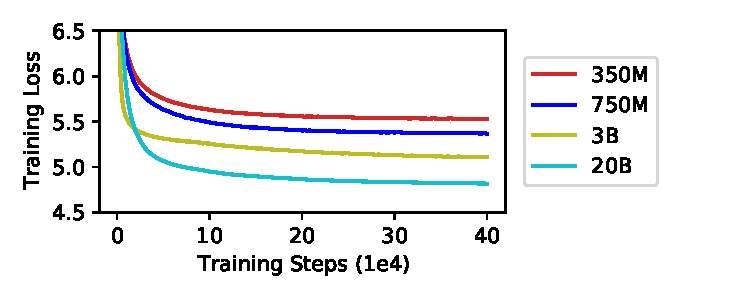
\includegraphics[width=0.64\textwidth]{figures/losscurve.pdf}
\caption{Effects of scaling \bdraw models of different sizes.
We show zero-shot FID scores \textit{(left)} on MS-COCO (2014) and the training loss curves of the corresponding models \textit{(right)}.}
\label{tabs:scaling_results}
\end{figure}
\begin{figure}[ht!]
        \centering                     
        \footnotesize
    \setlength\tabcolsep{2pt}
    \vspace{-0.5in}
    \begin{tabular}{cccc}
        \textbf{\bdraw-350M} & \textbf{\bdraw-750M} & \textbf{\bdraw-3B} & \textbf{\bdraw-20B} \\[2mm]

        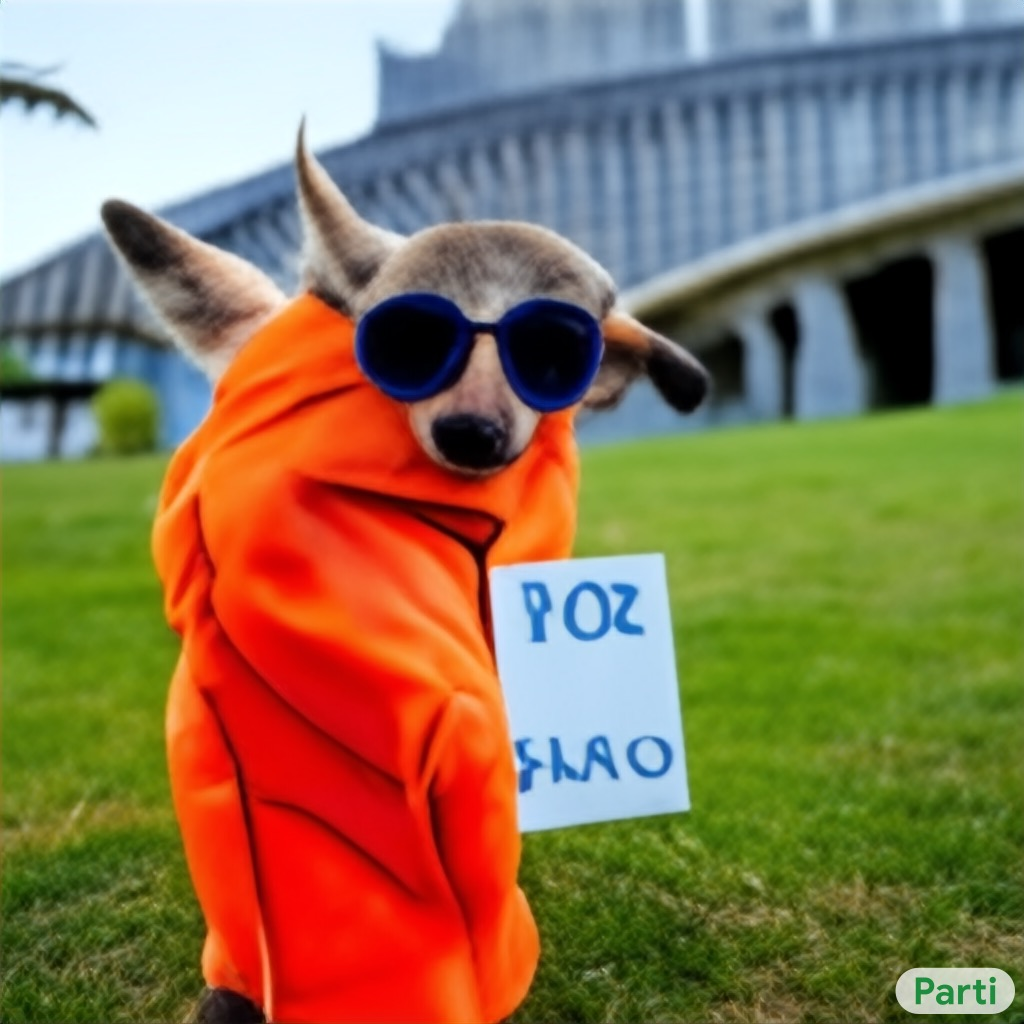
\includegraphics[width=0.24\textwidth]{figures/scaling_comparison/kangaroo_0.jpg} &
        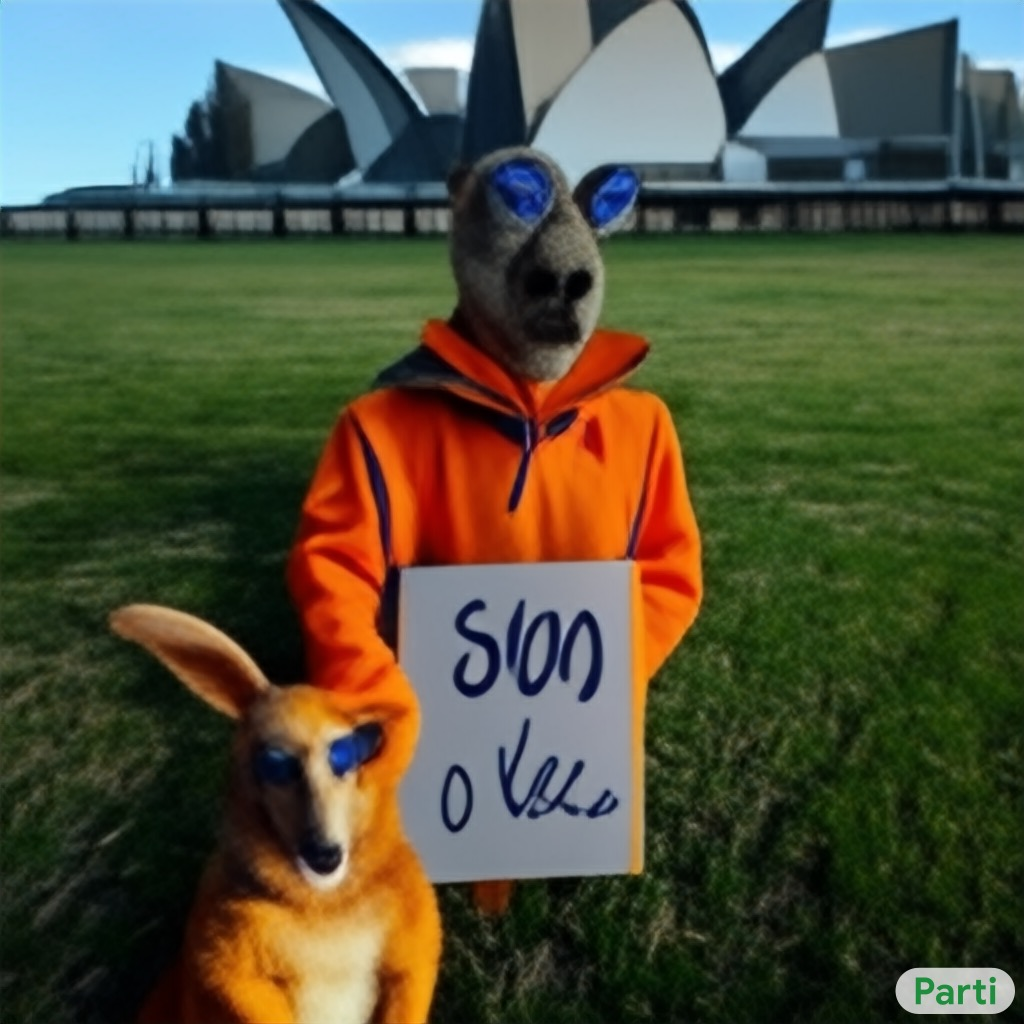
\includegraphics[width=0.24\textwidth]{figures/scaling_comparison/kangaroo_1.jpg} &
        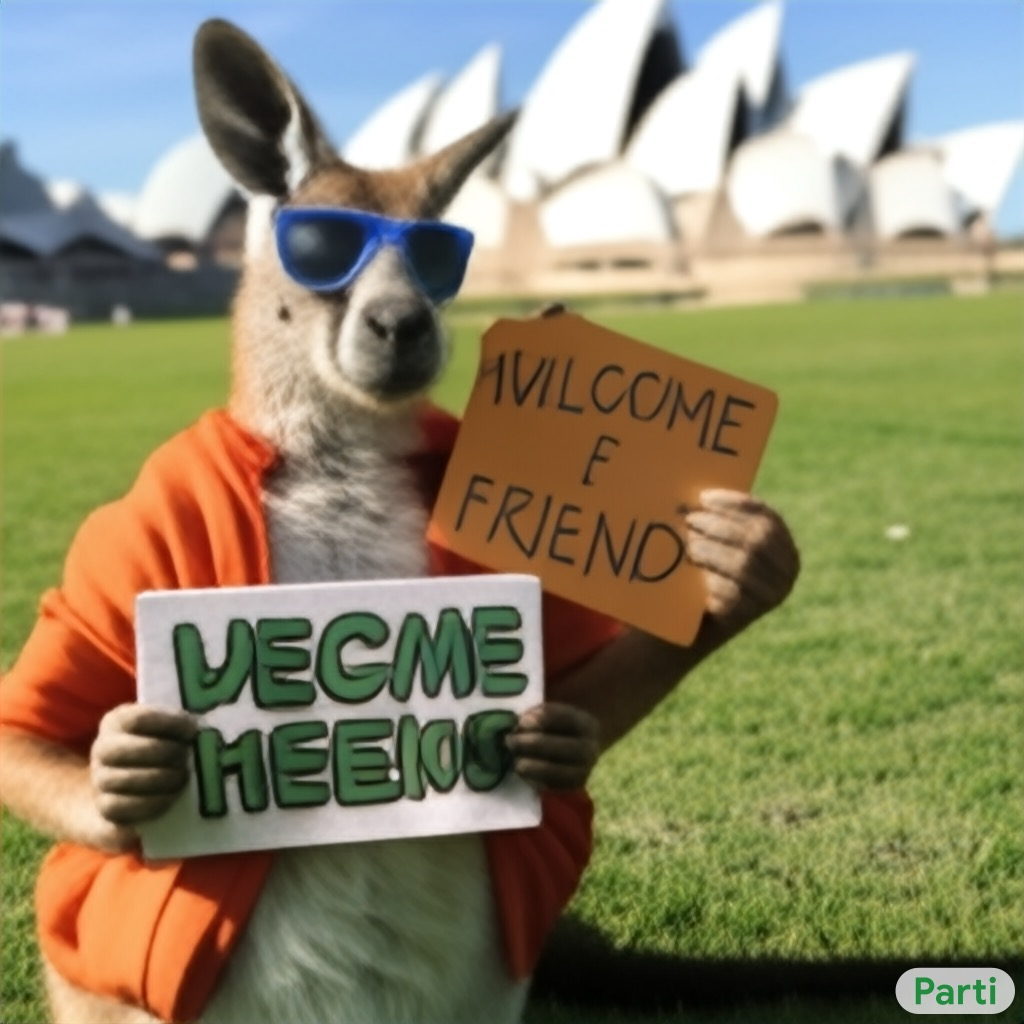
\includegraphics[width=0.24\textwidth]{figures/scaling_comparison/kangaroo_2.jpg} &
        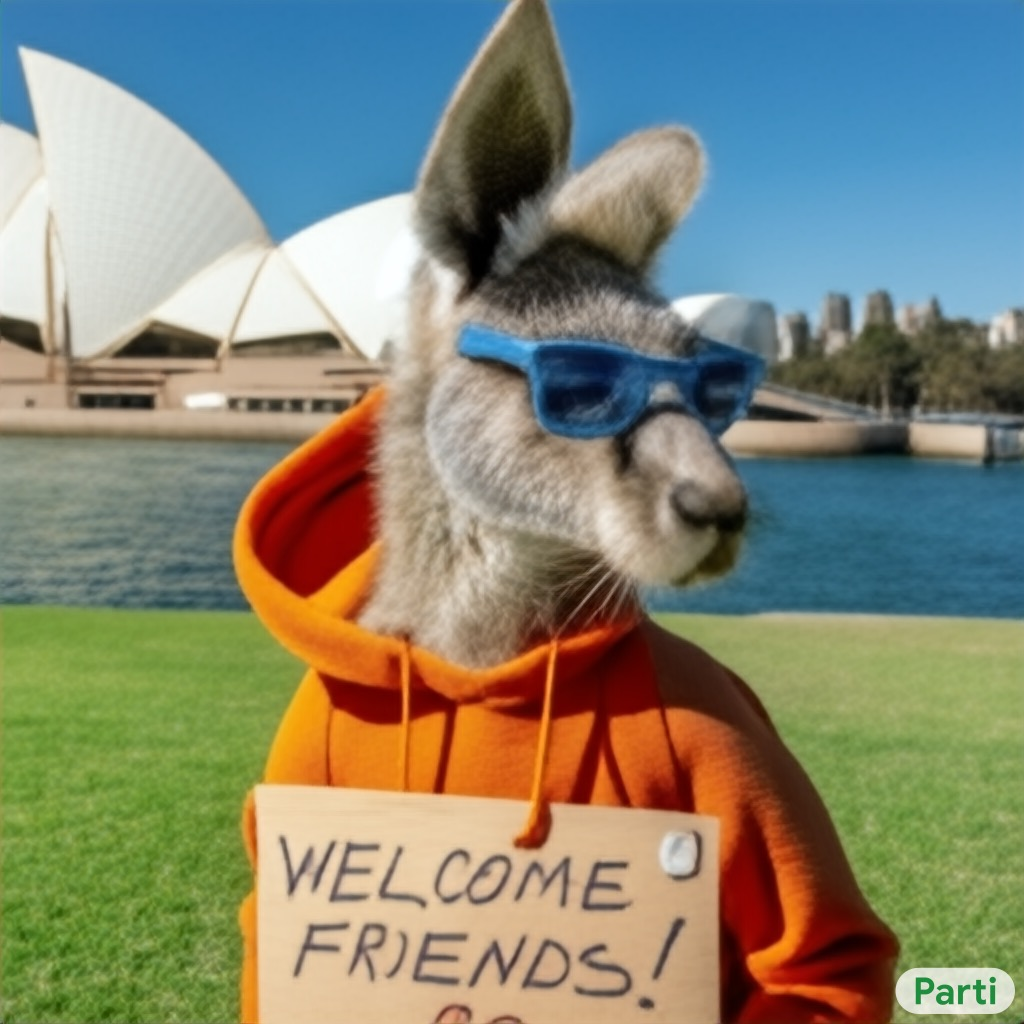
\includegraphics[width=0.24\textwidth]{figures/scaling_comparison/kangaroo_3.jpg}\vspace{1mm} \\
        \multicolumn{4}{c}{\small A portrait photo of a kangaroo wearing an orange hoodie and blue sunglasses standing on the grass} \\
        \multicolumn{4}{c}{\small in front of the Sydney Opera House holding a sign on the chest that says Welcome Friends!}\vspace{3mm}\\

        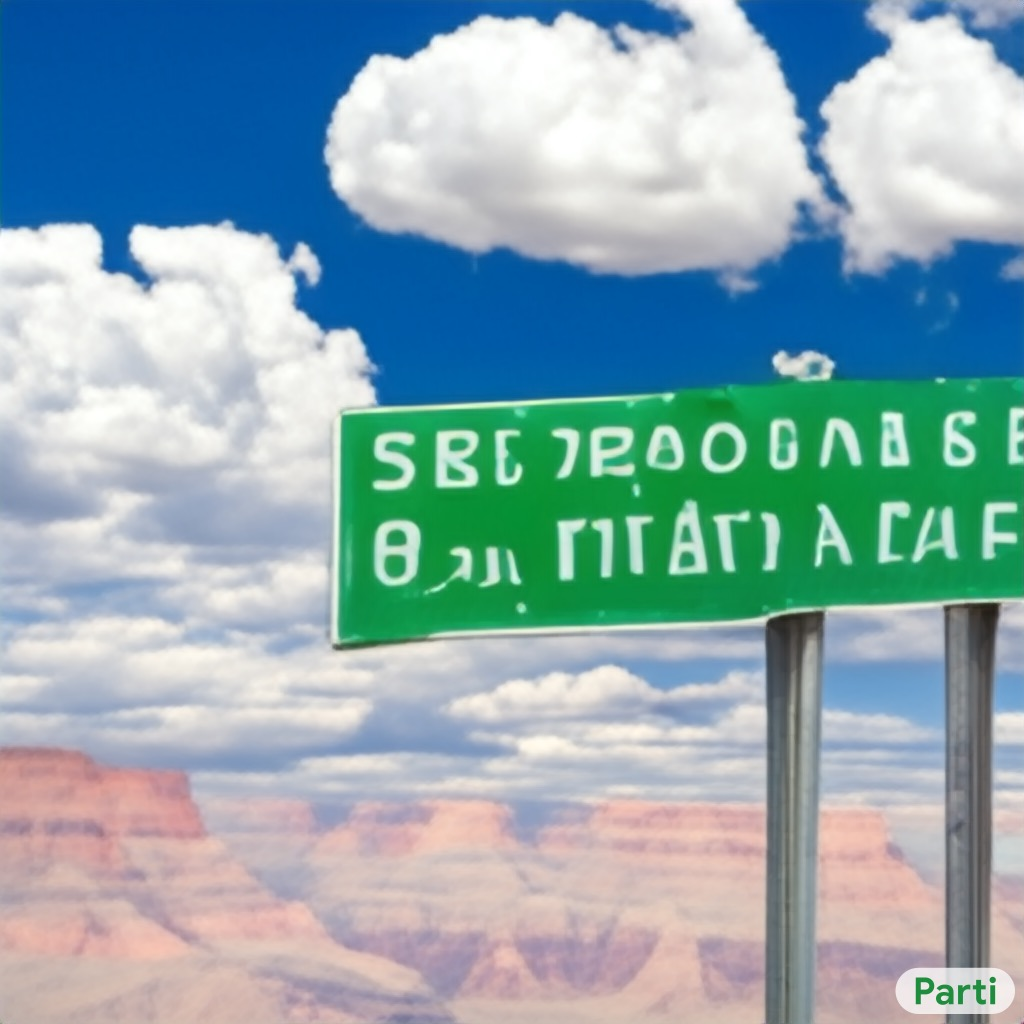
\includegraphics[width=0.24\textwidth]{figures/scaling_comparison/dl_0.jpg} &
        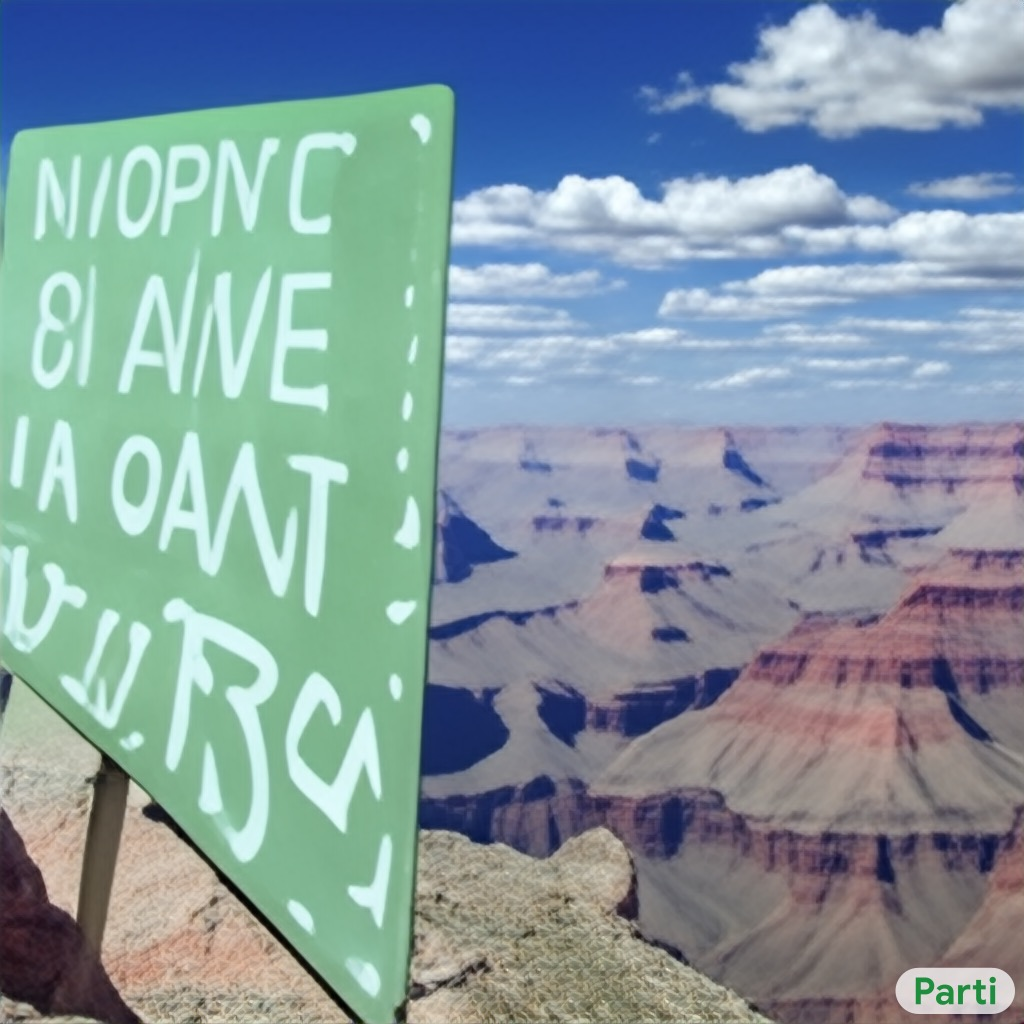
\includegraphics[width=0.24\textwidth]{figures/scaling_comparison/dl_1.jpg} &
        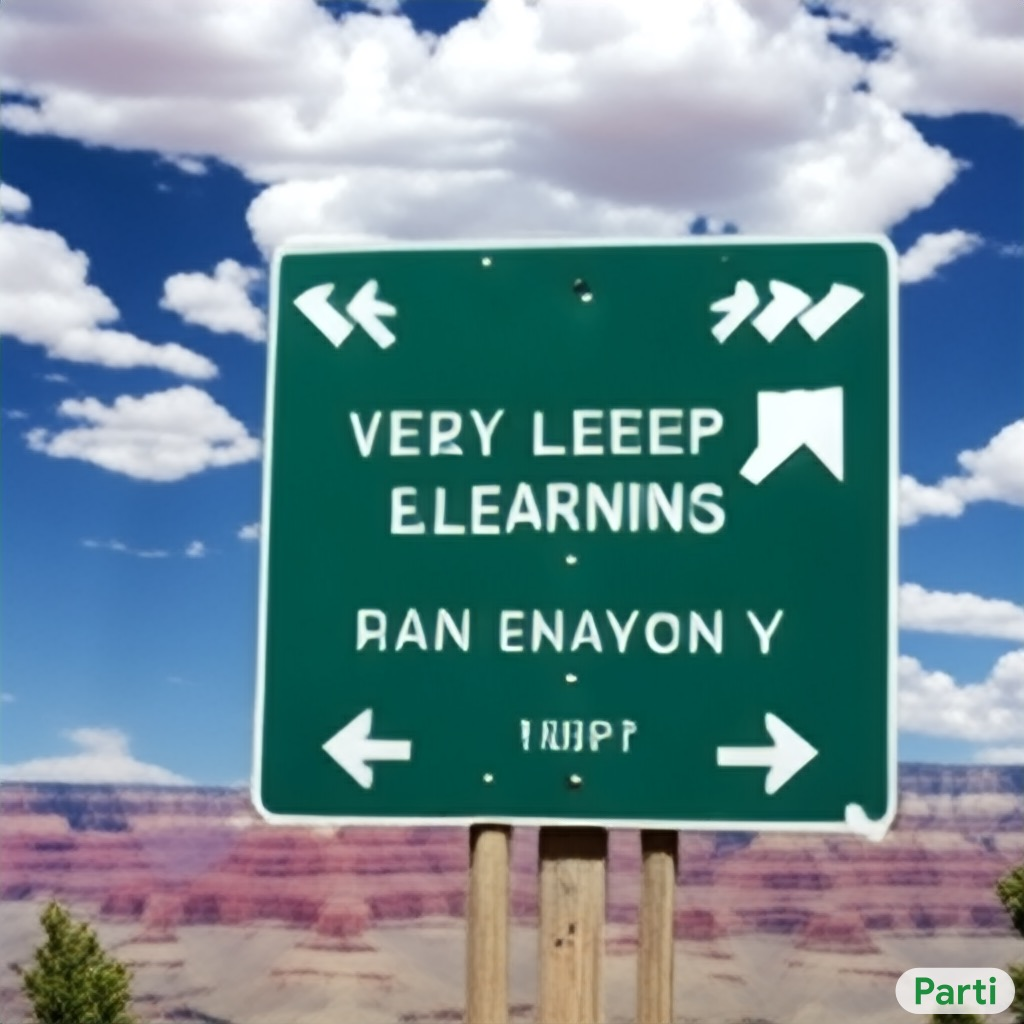
\includegraphics[width=0.24\textwidth]{figures/scaling_comparison/dl_2.jpg} &
        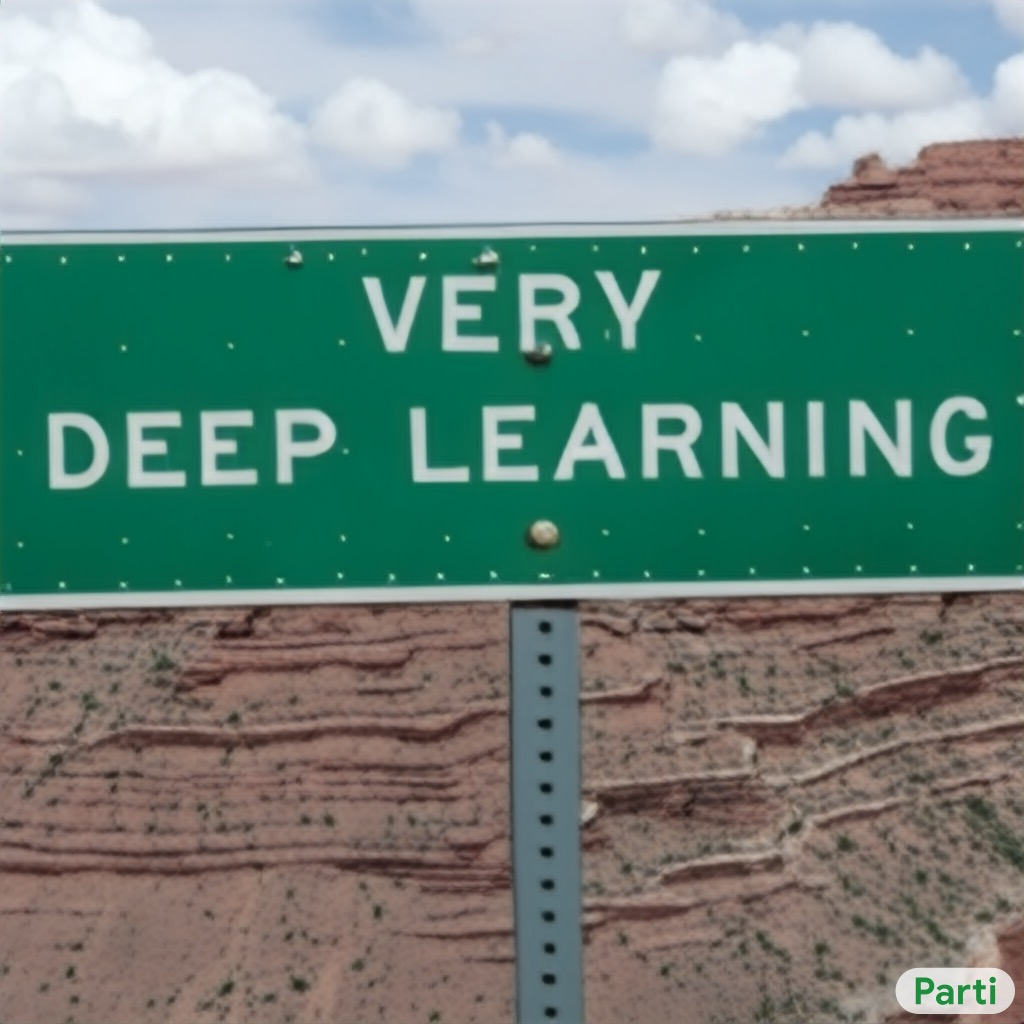
\includegraphics[width=0.24\textwidth]{figures/scaling_comparison/dl_3.jpg}\vspace{1mm} \\
        \multicolumn{4}{c}{\small A green sign that says "Very Deep Learning" and is at the edge of the Grand Canyon.}\\
        \multicolumn{4}{c}{\small Puffy white clouds are in the sky.}\vspace{3mm}\\

        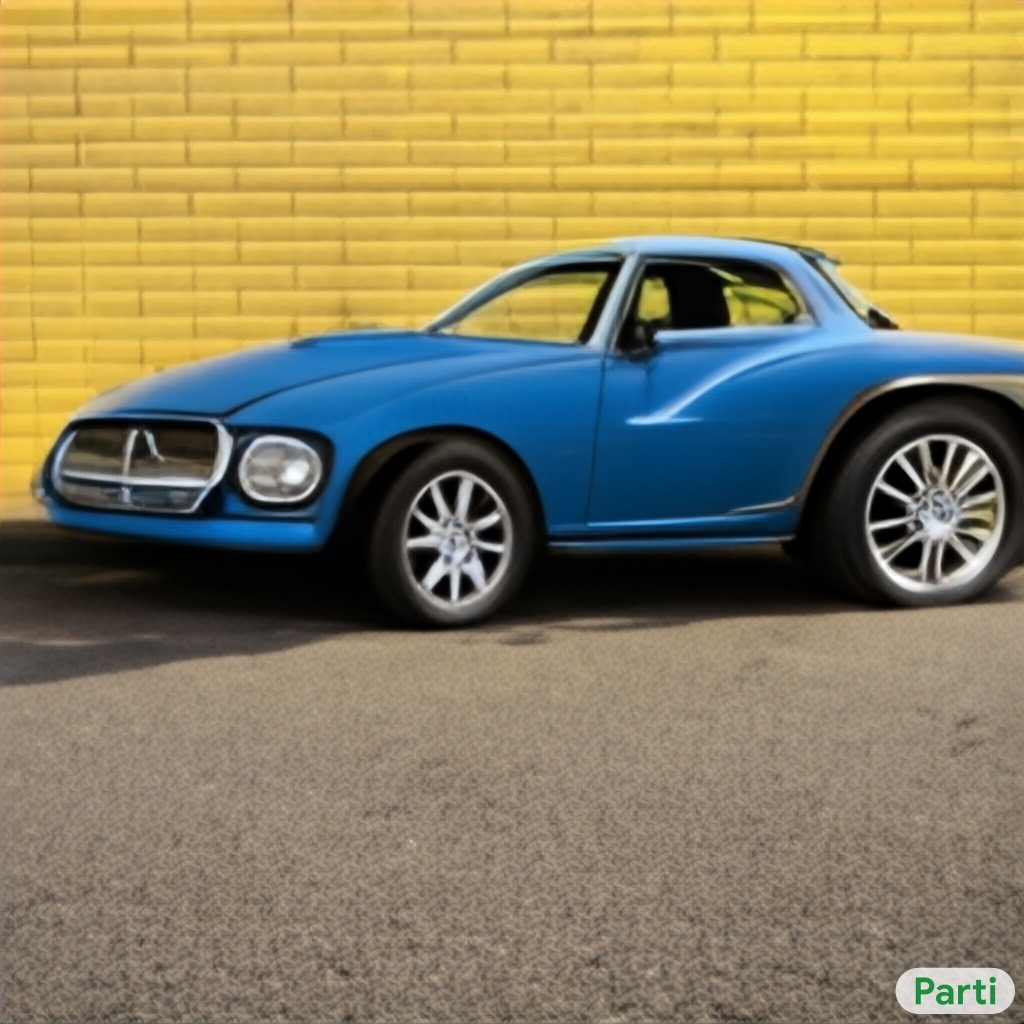
\includegraphics[width=0.24\textwidth]{figures/scaling_comparison/p356_0.jpg} &
        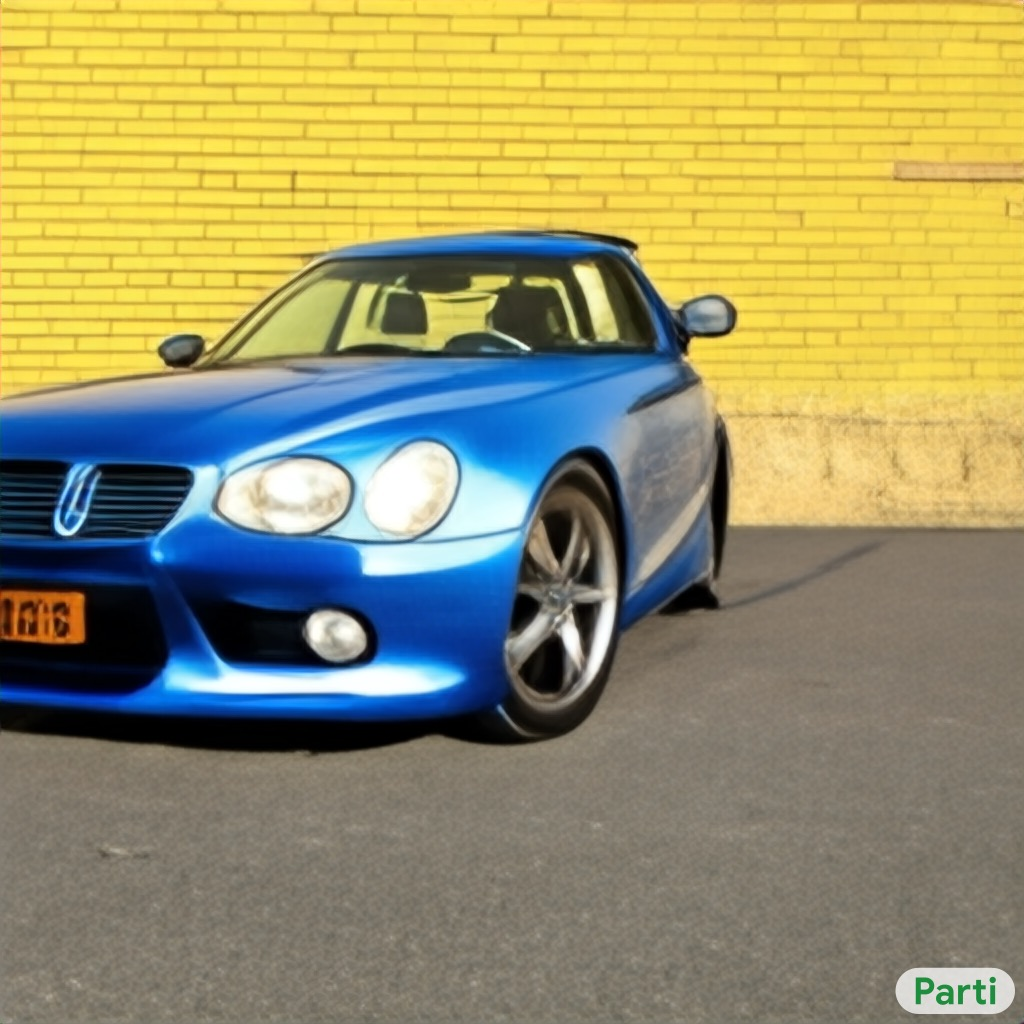
\includegraphics[width=0.24\textwidth]{figures/scaling_comparison/p356_1.jpg} &
        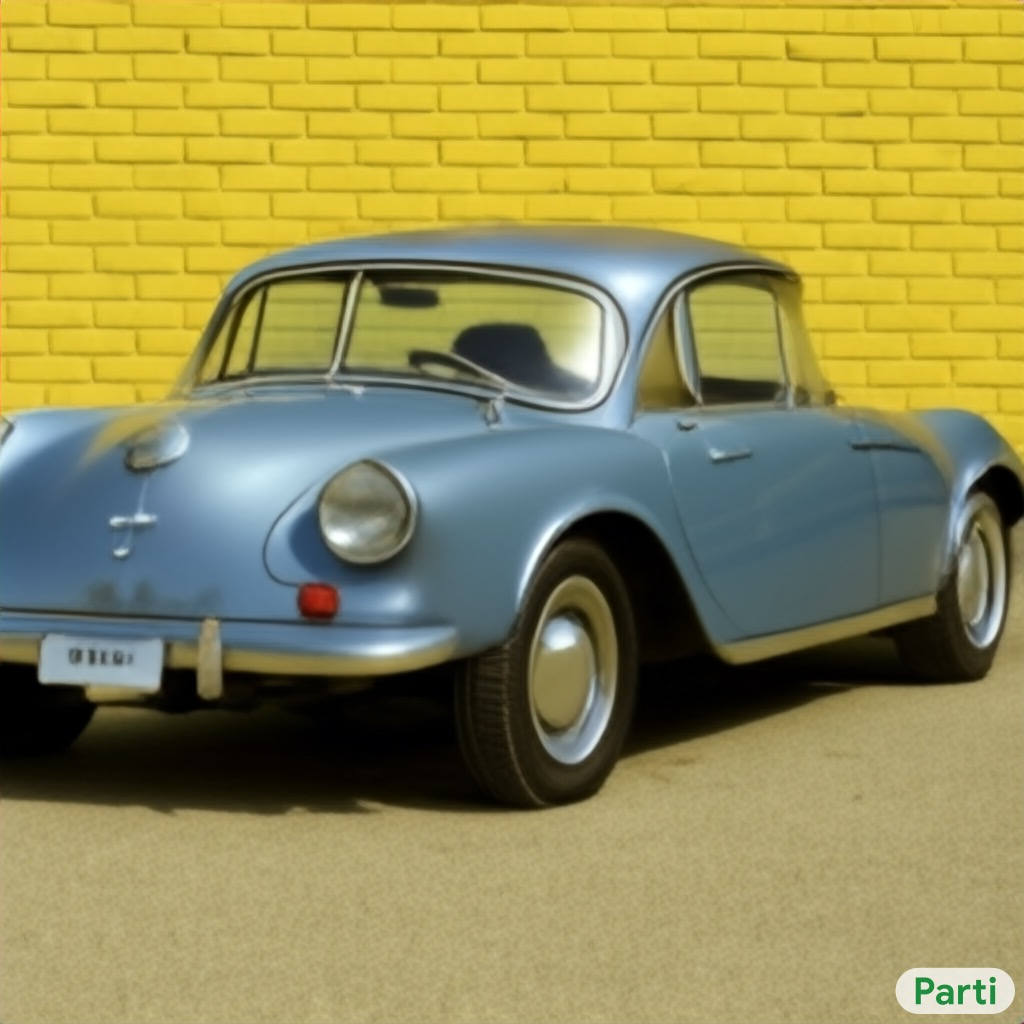
\includegraphics[width=0.24\textwidth]{figures/scaling_comparison/p356_2.jpg} &
        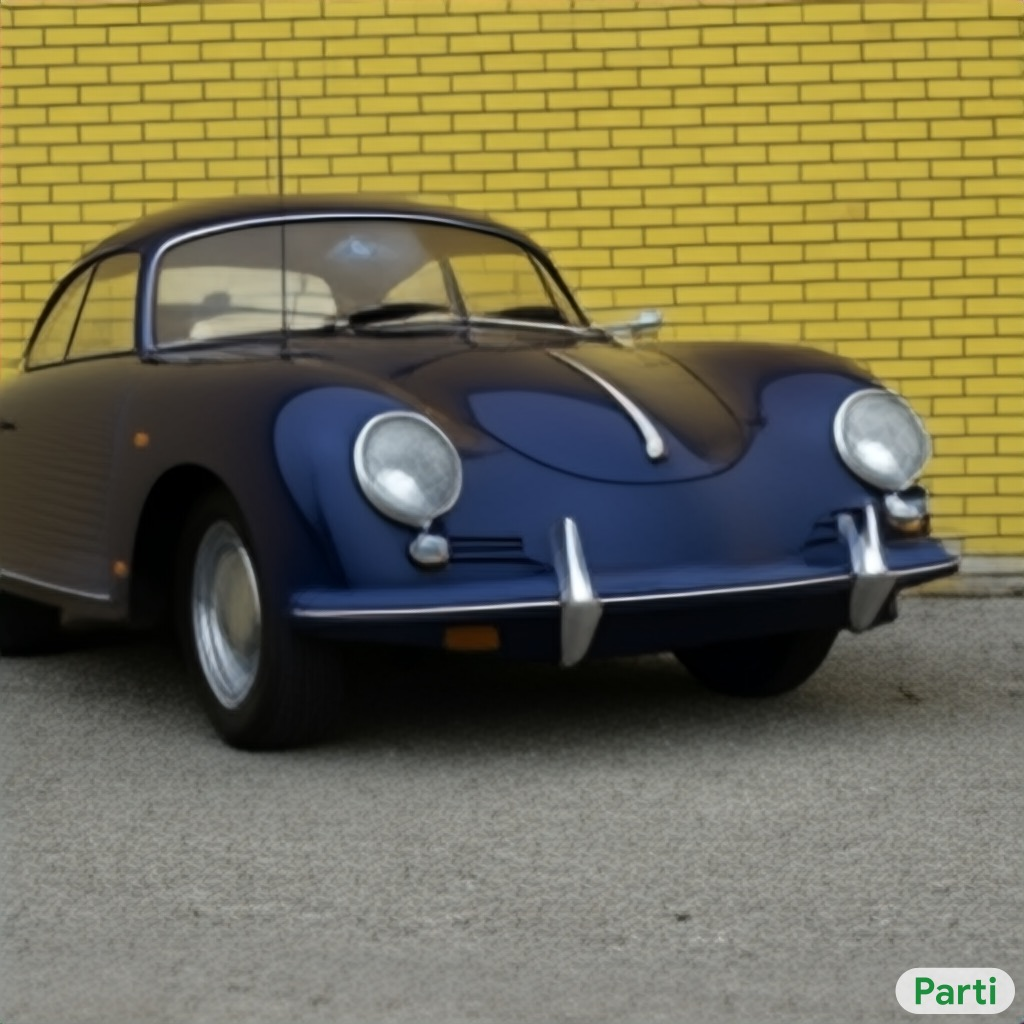
\includegraphics[width=0.24\textwidth]{figures/scaling_comparison/p356_3.jpg}\vspace{1mm} \\
        \multicolumn{4}{c}{\small A blue Porsche 356 parked in front of a yellow brick wall.}\vspace{3mm}\\

        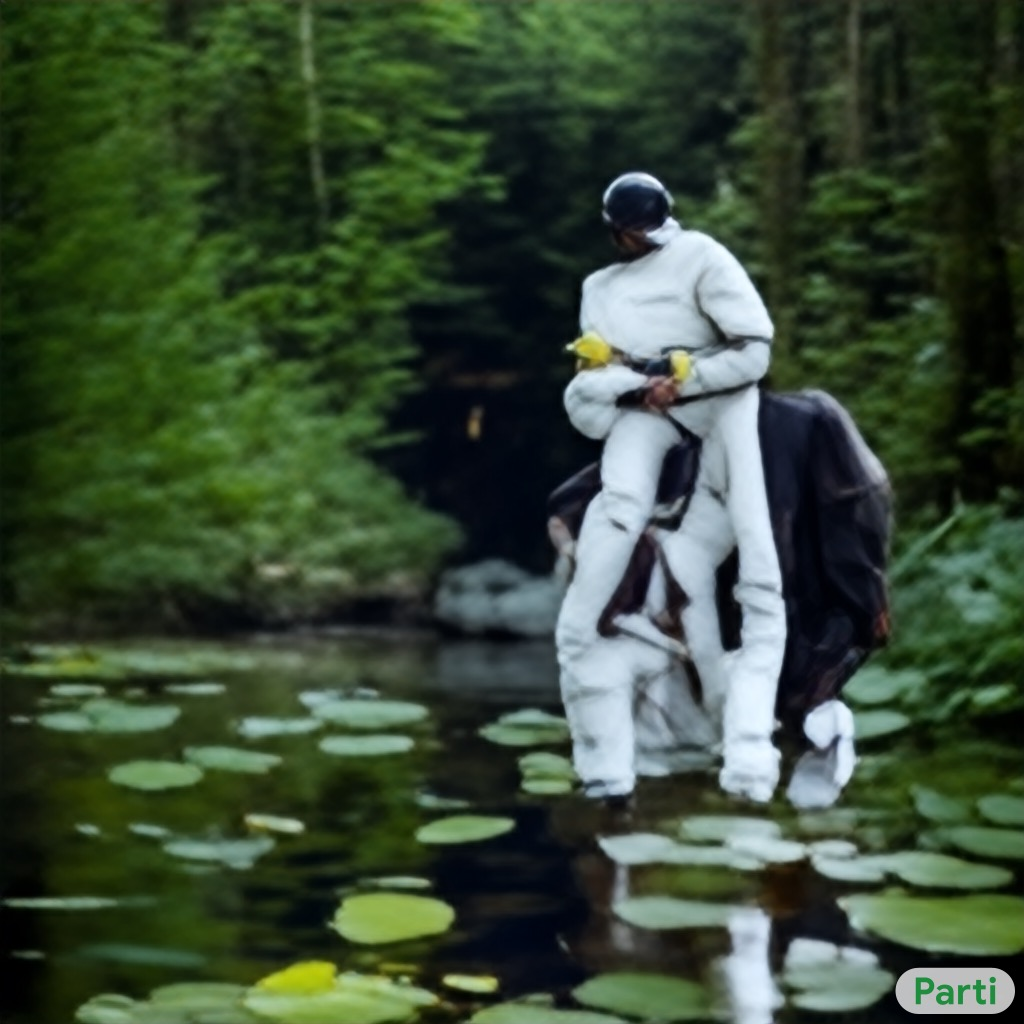
\includegraphics[width=0.24\textwidth]{figures/scaling_comparison/astronaut_0.jpg} &
        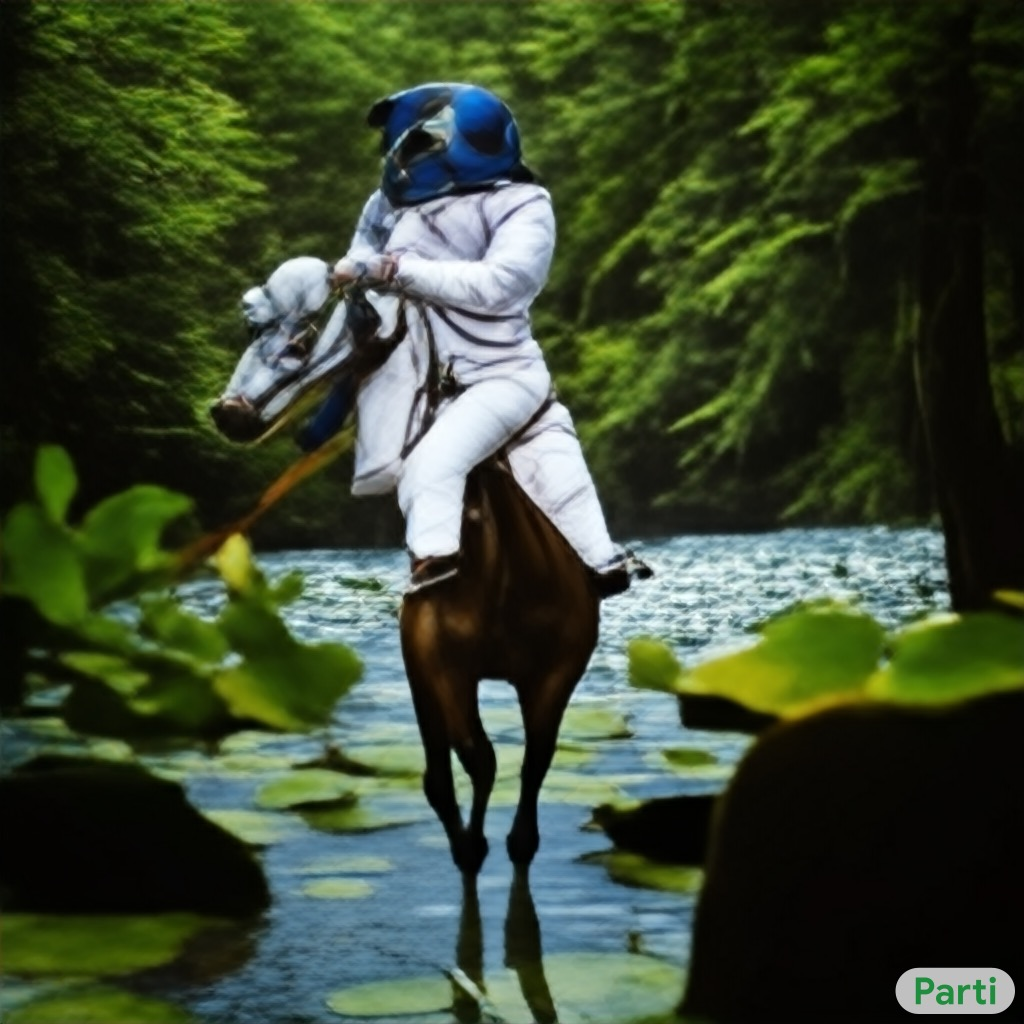
\includegraphics[width=0.24\textwidth]{figures/scaling_comparison/astronaut_1.jpg} &
        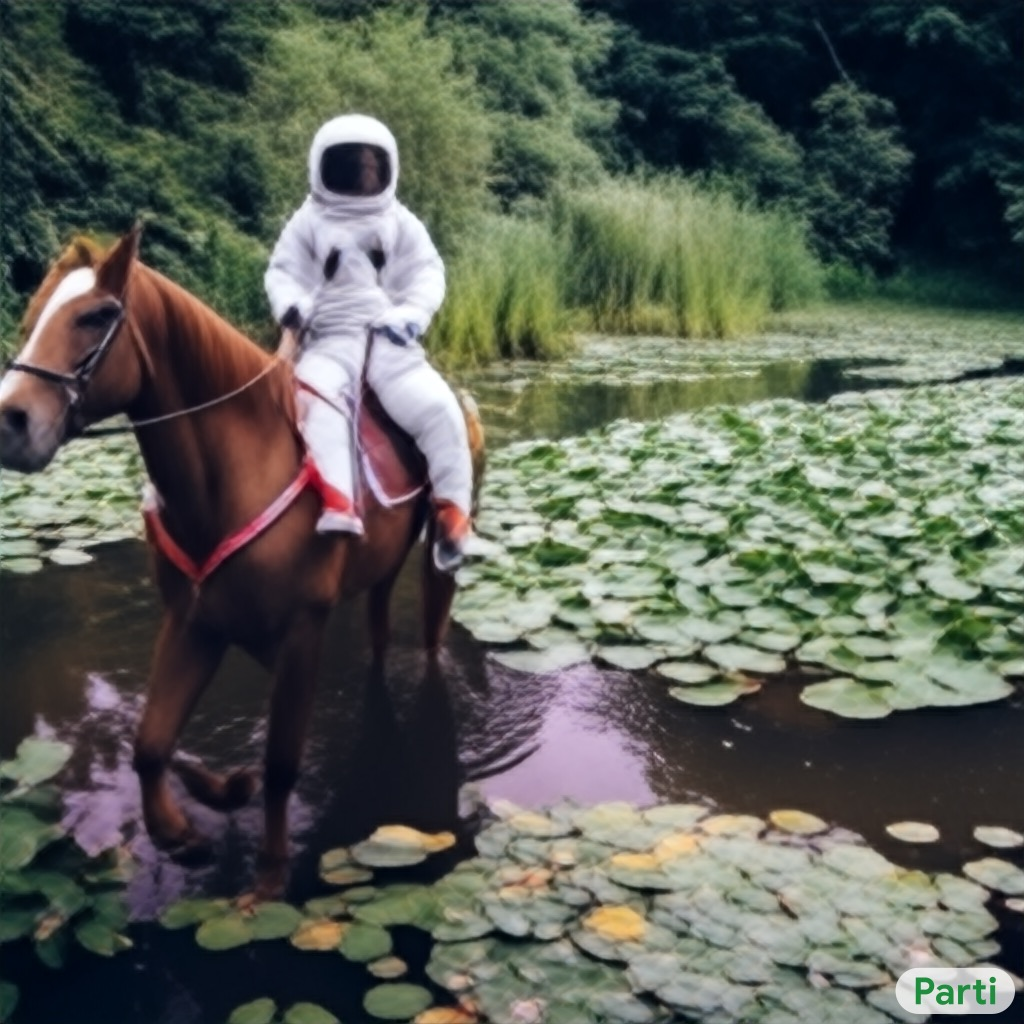
\includegraphics[width=0.24\textwidth]{figures/scaling_comparison/astronaut_2.jpg} &
        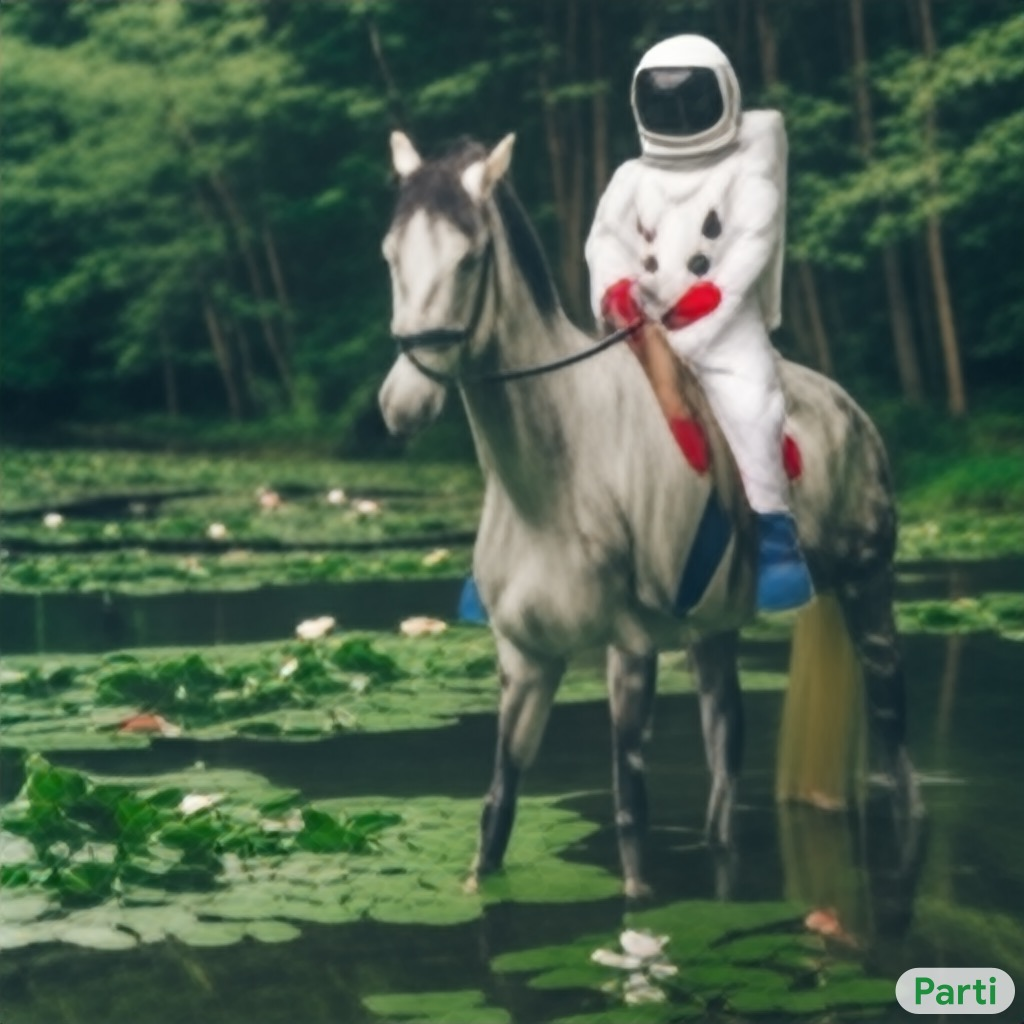
\includegraphics[width=0.24\textwidth]{figures/scaling_comparison/astronaut_3.jpg}\vspace{1mm} \\
        \multicolumn{4}{c}{\small A photo of an astronaut riding a horse in the forest. There is a river in front of them with water lilies.}\vspace{3mm}\\

        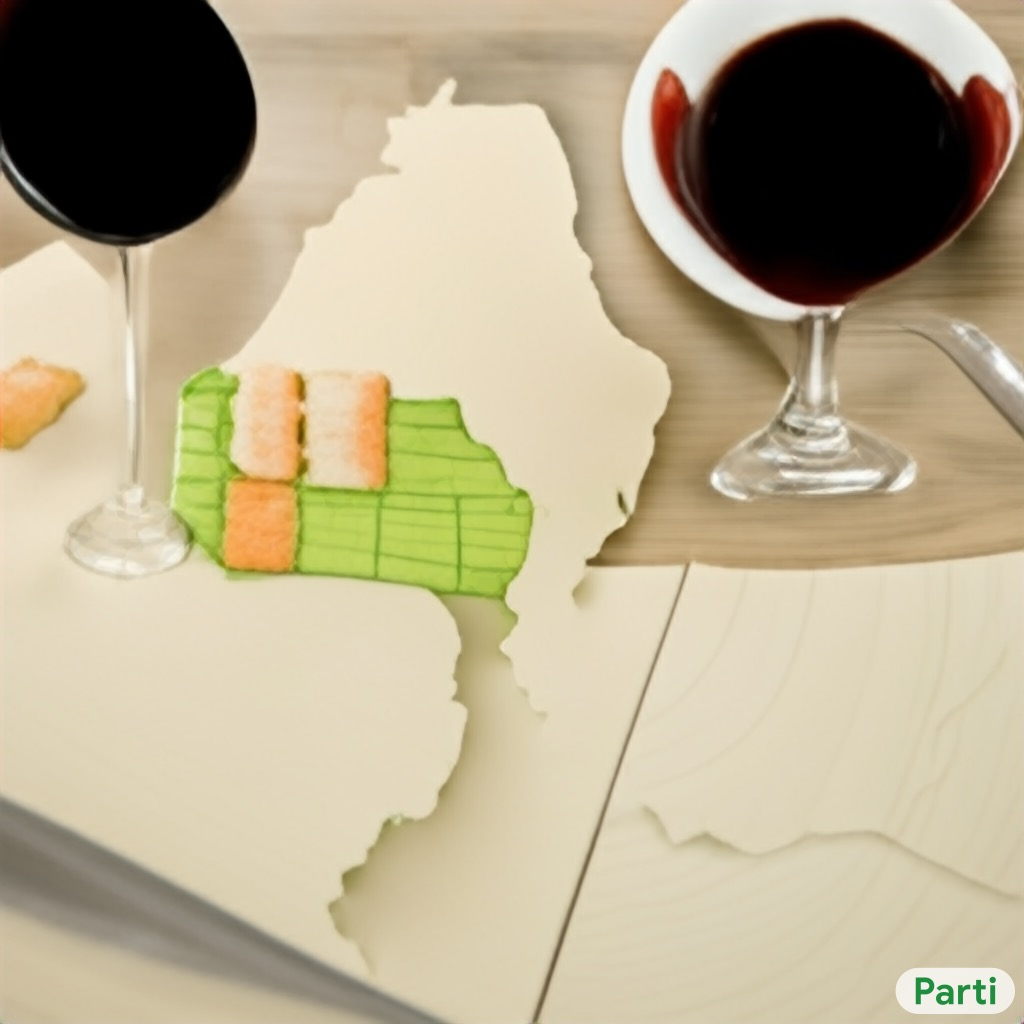
\includegraphics[width=0.24\textwidth]{figures/scaling_comparison/map_0.jpg} &
        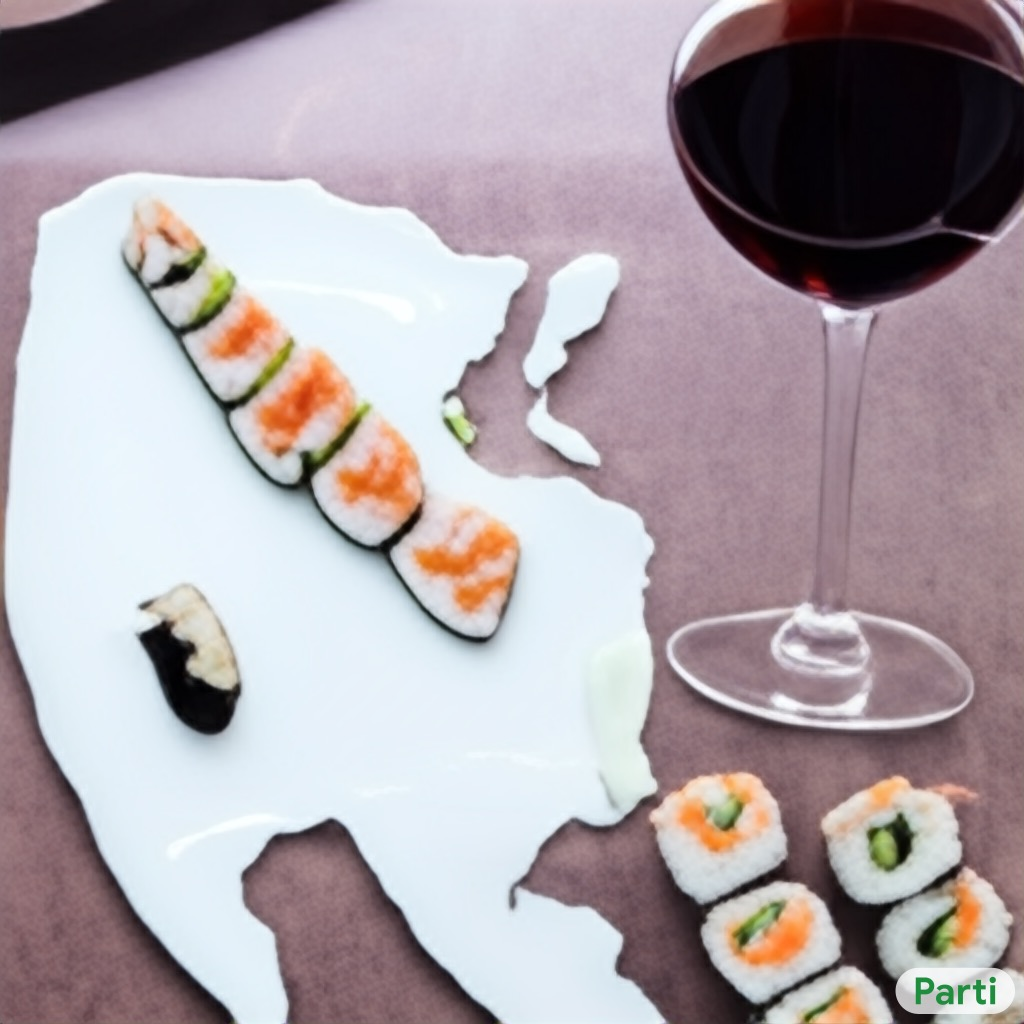
\includegraphics[width=0.24\textwidth]{figures/scaling_comparison/map_1.jpg} &
        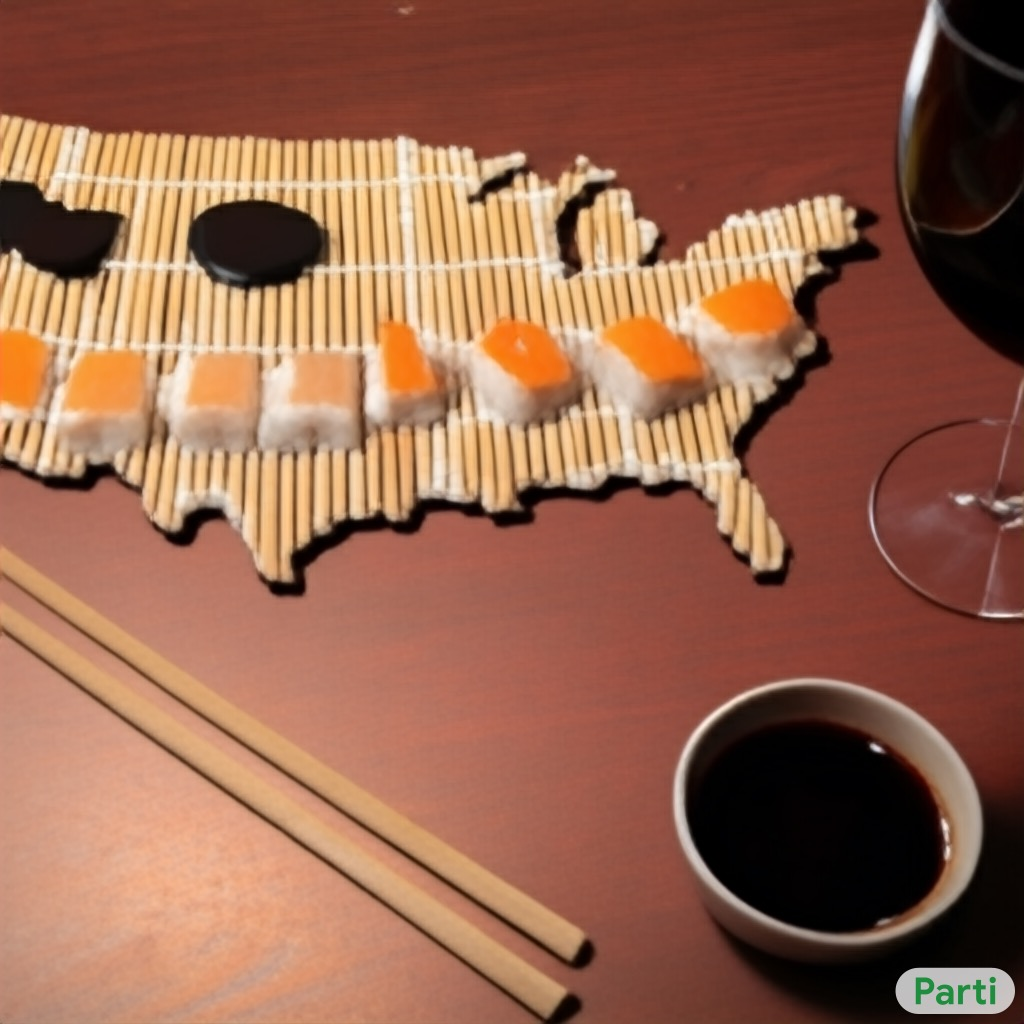
\includegraphics[width=0.24\textwidth]{figures/scaling_comparison/map_2.jpg} &
        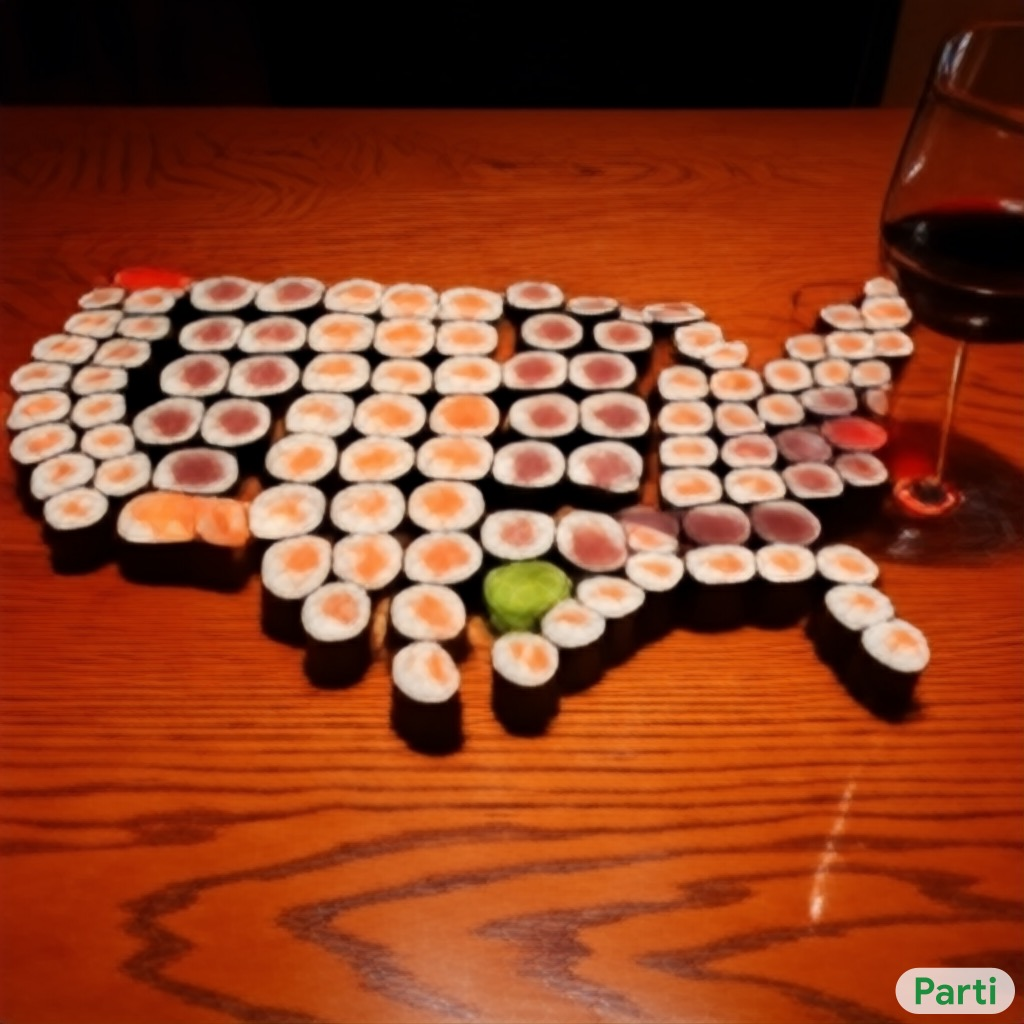
\includegraphics[width=0.24\textwidth]{figures/scaling_comparison/map_3.jpg}\vspace{1mm} \\
        \multicolumn{4}{c}{\small A map of the United States made out of sushi. It is on a table next to a glass of red wine.} \\
    \end{tabular} 
    \caption{Qualitative comparison of top-1 images sampled from \bdraw models of increasing sizes (350M, 750M, 3B, 20B). All \bdraw models sample 16 images per text prompt and rerank using the same CoCa model described in Section~\ref{secs:sampling_cf_coca}. We use prompts in the \bcpa{} benchmark (Section~\ref{secs:bcp}) to test \bcpstyle{World Knowledge}, \bcpstyle{Fine-grained Detail}, and \bcpstyle{Writing \& Symbols.}
    }
    \label{figs:scaling_comparison}
    \vspace{-0.15in}
\end{figure}
\textbf{Comparison of Model Scaling.} 
We compare four different model sizes of \bdraw, with parameter counts ranging from 350M, 750M to 3B and 20B, as shown in Table~\ref{tabs:bdraw_variants}. All four models are trained on the same mixture of datasets with the same image tokenizer and CoCa reranking model described in Section~\ref{secs:sampling_cf_coca}. 
Figure~\ref{tabs:scaling_results} summarizes the corresponding zero-shot FID scores on MS-COCO (2014). \bdraw models are trained with next token prediction loss for text-to-image generation, using softmax cross-entropy loss over a 8192-vocab image codebook. The loss is averaged by 1024 (the total output length) image tokens per example. We observe better training loss as well as zero-shot FID on MS-COCO when we scale up the model. Specifically, a significant quality jump is achieved by scaling model from 750M to 3B; furthermore, the 20B model outperforms 3B model in more challenging prompts (\eg, text rendering).
We highlight qualitatively how these models perform visually in Figures \ref{figs:scaling_comparison} and \ref{figs:scaling_bcp}, using challenging prompts from the \bcpa{} benchmark (see Section~\ref{secs:evaluations_bcp}).


\subsection{Results on \bcp}
\label{secs:evaluations_bcp}

\begin{figure}[tbh!]
    \centering
    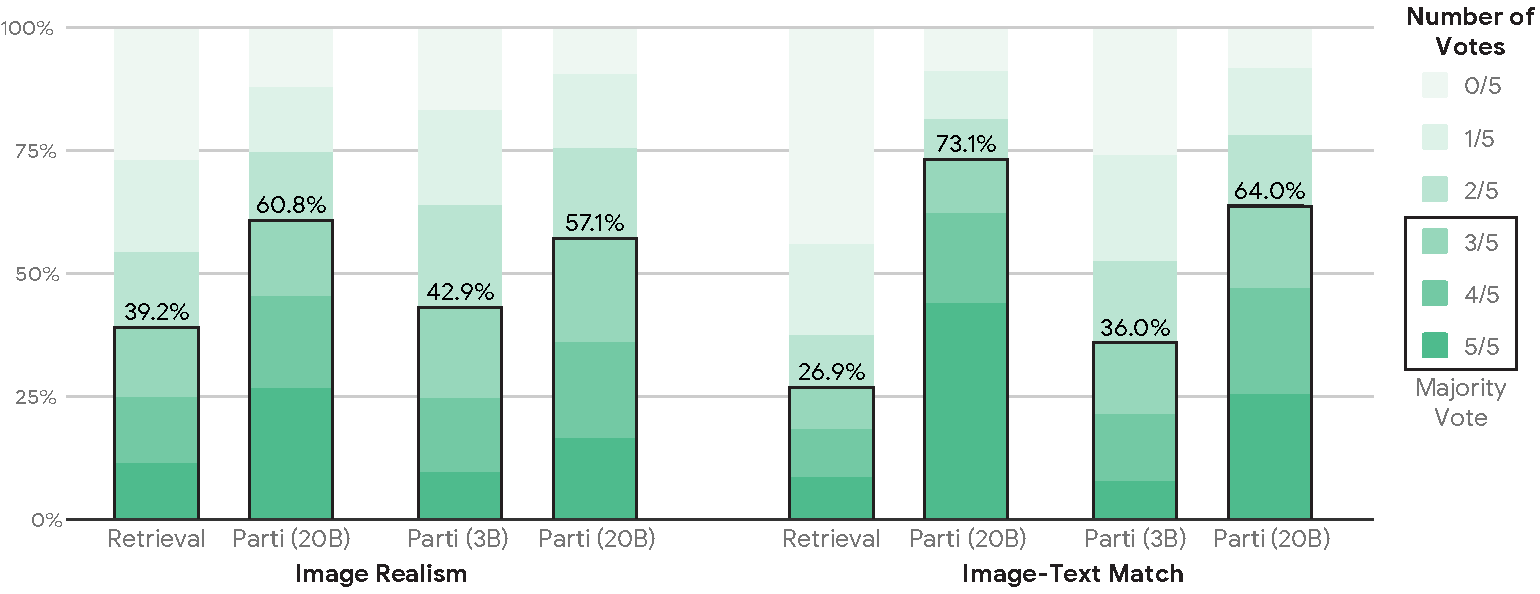
\includegraphics[width=1.0\textwidth]{figures/human_evals_bcp.pdf}
    \caption{Human evaluation results on \bcp.}
    \label{fig:human_evals_bcp}
\end{figure}

\textbf{Human Evaluations.} 
In addition to MS-COCO, we also conduct human evaluations on the \bcpa{} benchmark, comparing our 20B model against the 3B variant and the Retrieval baseline. Figure~\ref{fig:human_evals_bcp} shows that the 20B model is clearly preferred by annotators over the retrieval baseline both in terms of image realism (63.2\%) and image-text match (75.9\%). These results offer a complementary view to the comparison in Figure~\ref{fig:human_evals_coco}: on the much more challenging \bcpa{} benchmark (Section~\ref{secs:bcp}), the retrieval baseline was unable produce matching outputs for many prompts. The 3B model closes the gap but the 20B is still preferred in terms of image realism (56.8\%) and image-text match (62.7\%).


\begin{figure}[ht!]
    \centering
    \footnotesize
    \setlength\tabcolsep{2pt}
    \begin{tabular}{>{\centering\arraybackslash}p{0.5\textwidth}>{\centering\arraybackslash}p{0.5\textwidth}}
        \textbf{Categories} & \textbf{Challenge Aspects} \\
        \vspace{-0.1in}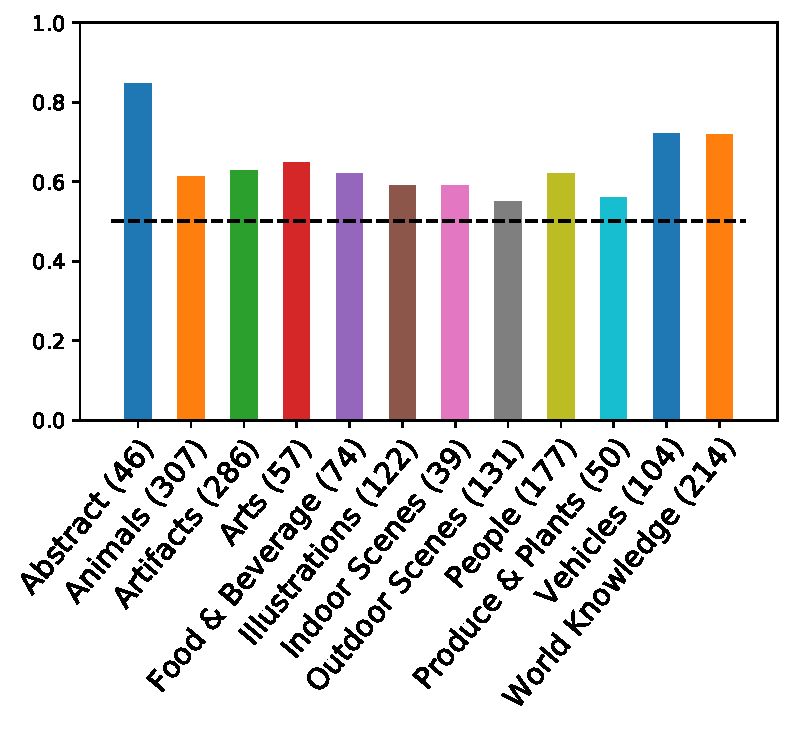
\includegraphics[width=0.48\textwidth]{figures/bcp_charts/bcp_20b_3b_breakdown_category_language.pdf} &
        \vspace{-0.1in}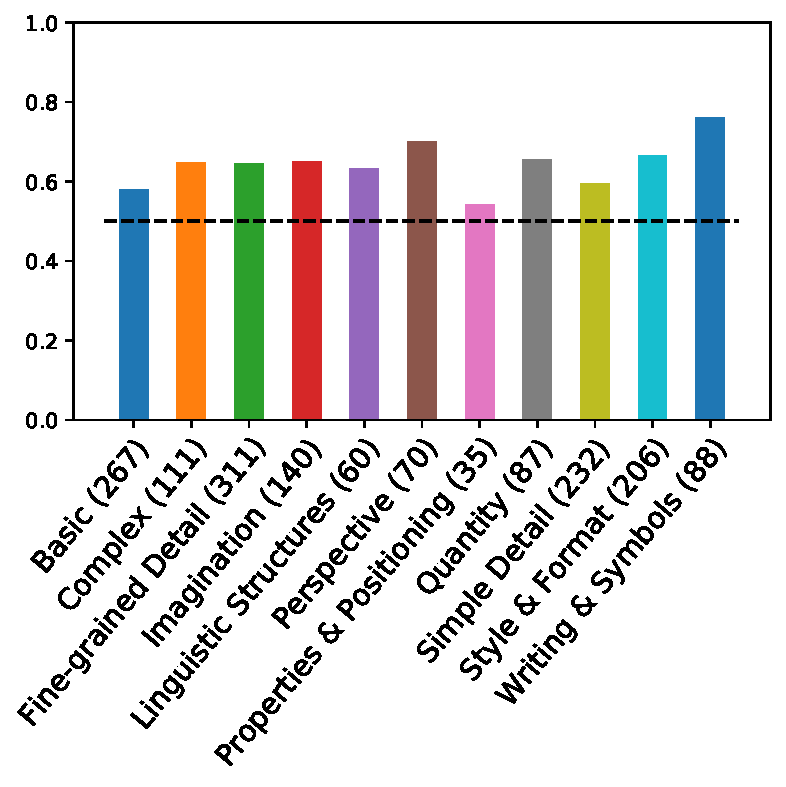
\includegraphics[width=0.48\textwidth]{figures/bcp_charts/bcp_20b_3b_breakdown_complexity_language.pdf} \vspace{1mm} \\
    \end{tabular} 
    \caption{
    Breakdown of human preferences of the \bdraw 20B model over the 3B model in terms of \bcpa{} categories ({\it left}) and challenge aspects ({\it right}). Each aspect is shown along with the number of prompts associated with it (e.g., the \textit{Abstract} category has \bcpabstractsize{} prompts).}
    \label{figs:bcp_20b_3b_language}
\end{figure}

\begin{figure}[ht!]
        \centering                     
        \footnotesize
    \setlength\tabcolsep{2pt}
    \vspace{-0.2in}
    \begin{tabular}{cccc}
        \textbf{\bdraw-350M} & \textbf{\bdraw-750M} & \textbf{\bdraw-3B} & \textbf{\bdraw-20B} \\[2mm]

        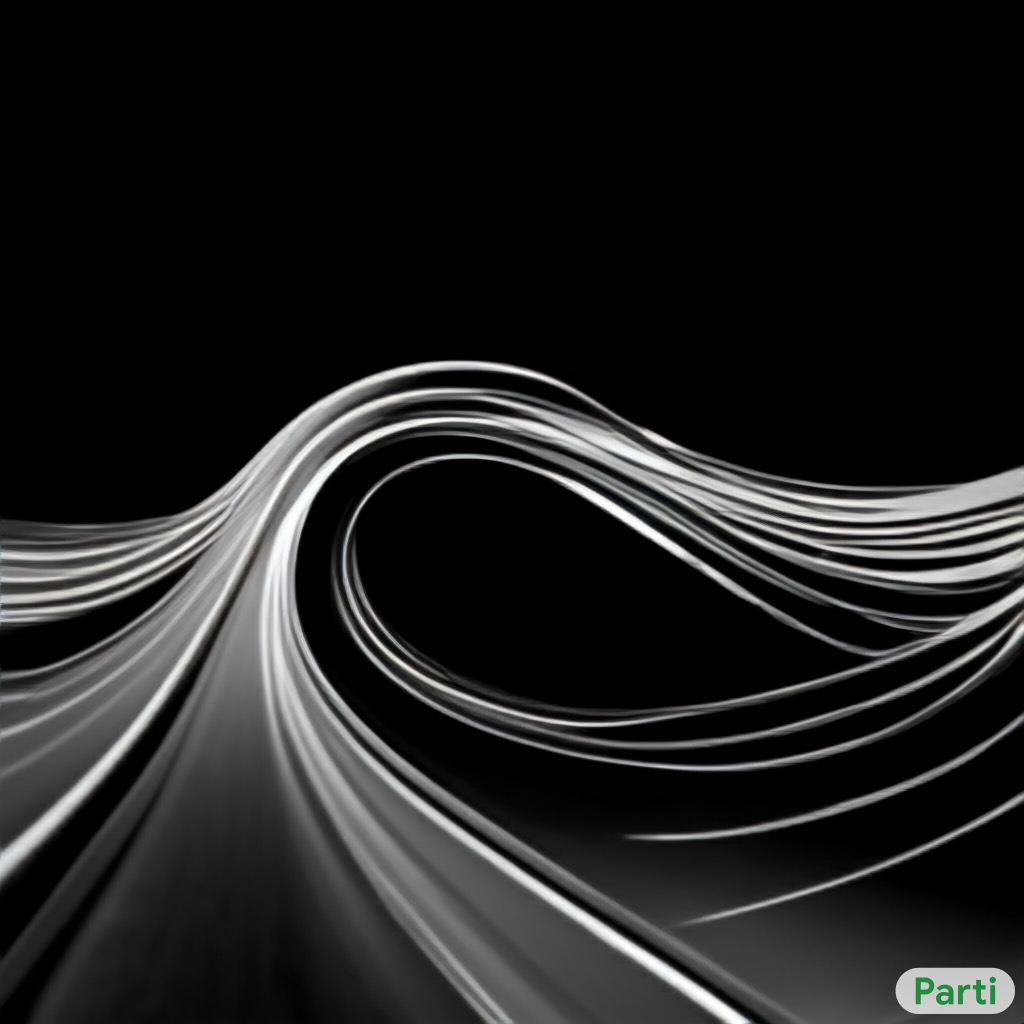
\includegraphics[width=0.24\textwidth]{figures/scaling_comparison/infinity_0.jpg} &
        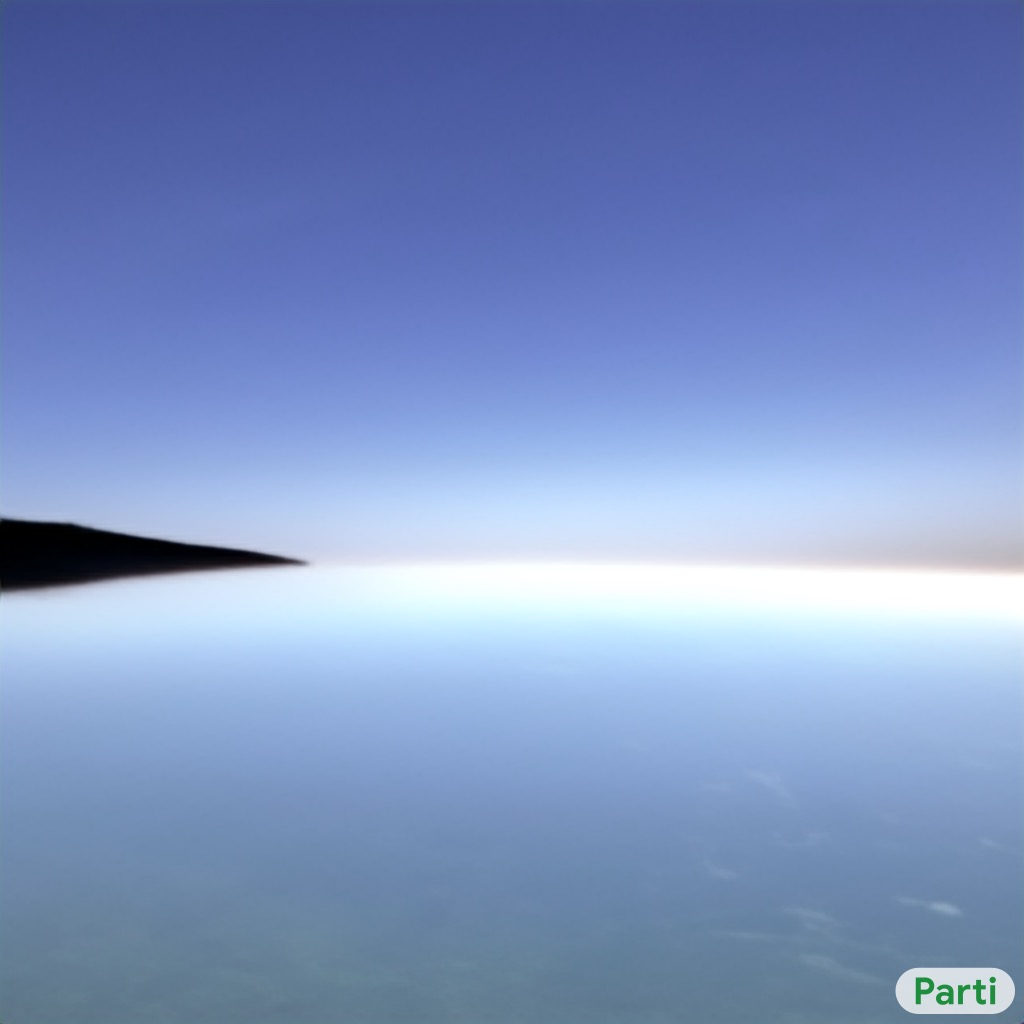
\includegraphics[width=0.24\textwidth]{figures/scaling_comparison/infinity_1.jpg} &
        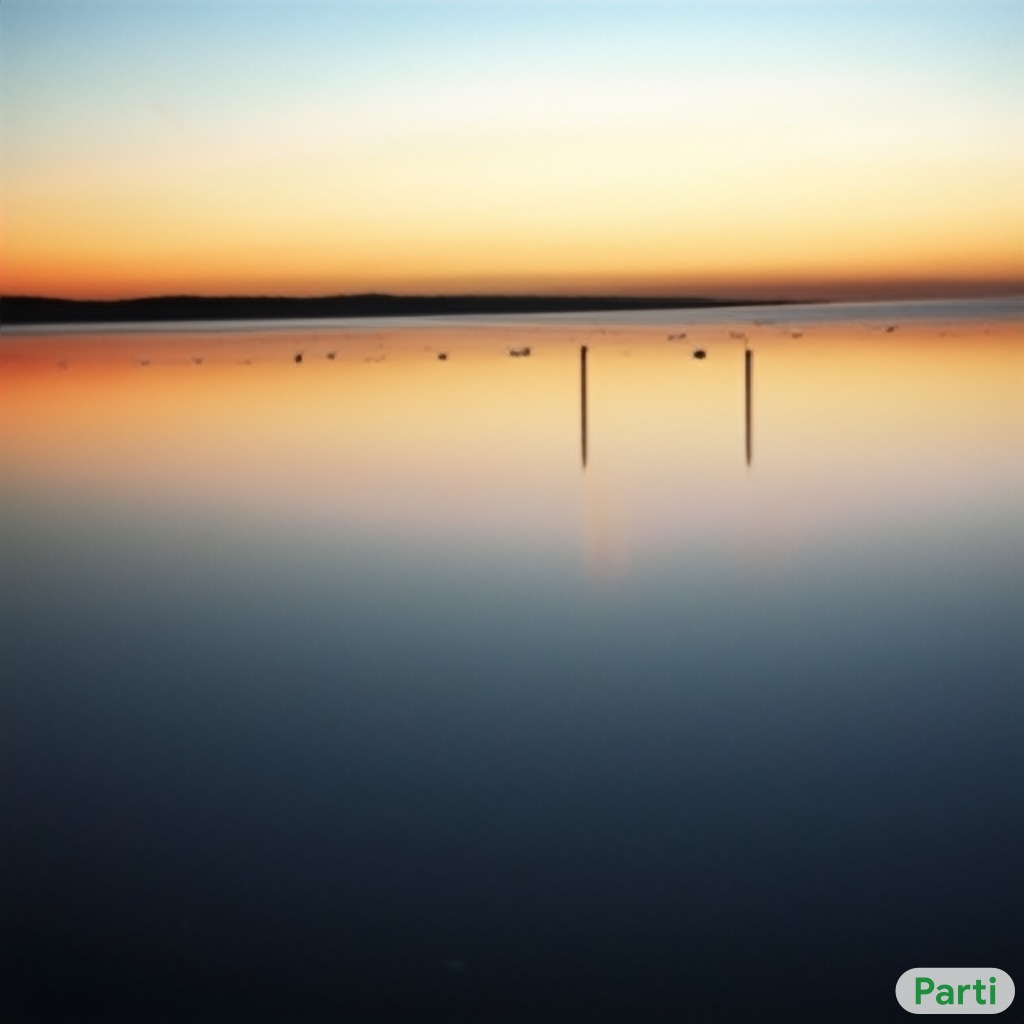
\includegraphics[width=0.24\textwidth]{figures/scaling_comparison/infinity_2.jpg} &
        
\includegraphics[width=0.24\textwidth]{figures/scaling_comparison/infinity_3.jpg}\vspace{1mm} \\
        \multicolumn{4}{c}{\small Infinity}\vspace{3mm}\\

        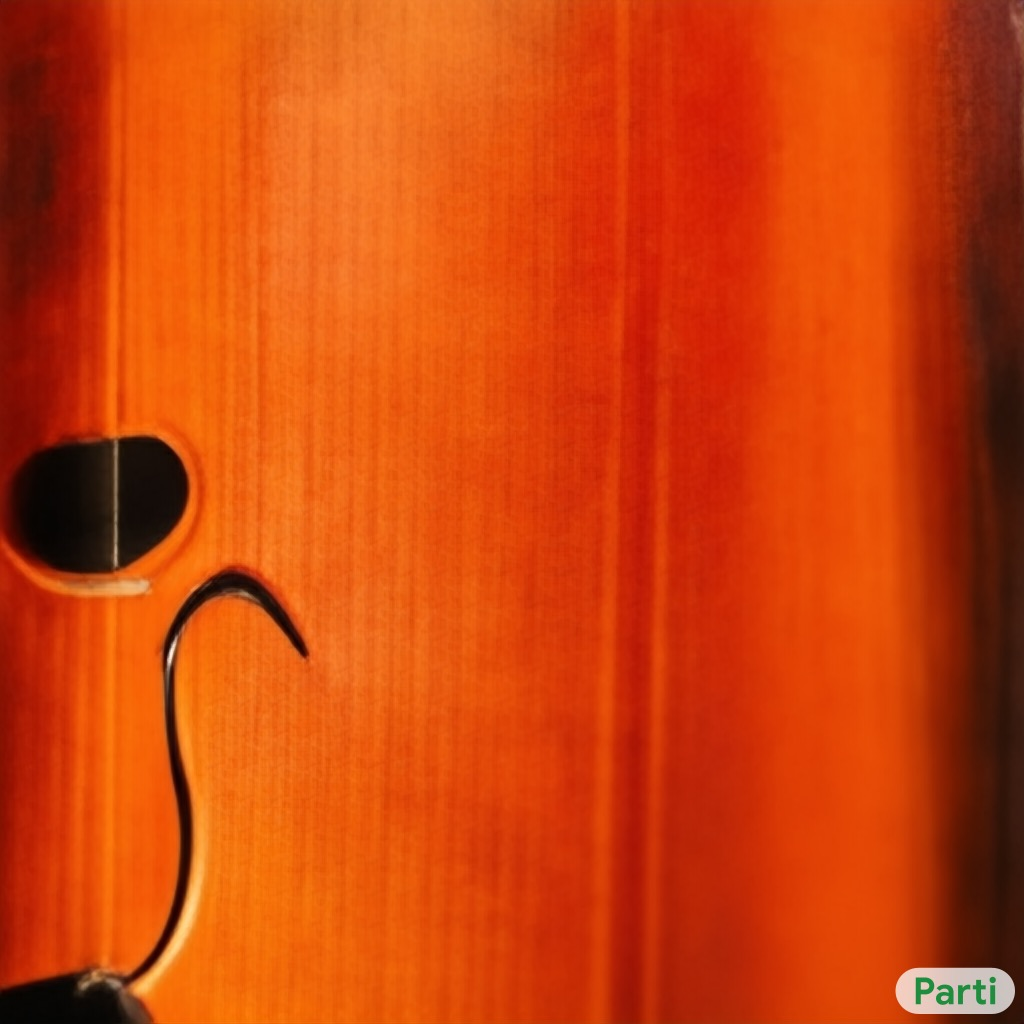
\includegraphics[width=0.24\textwidth]{figures/scaling_comparison/violin_0.jpg} &
        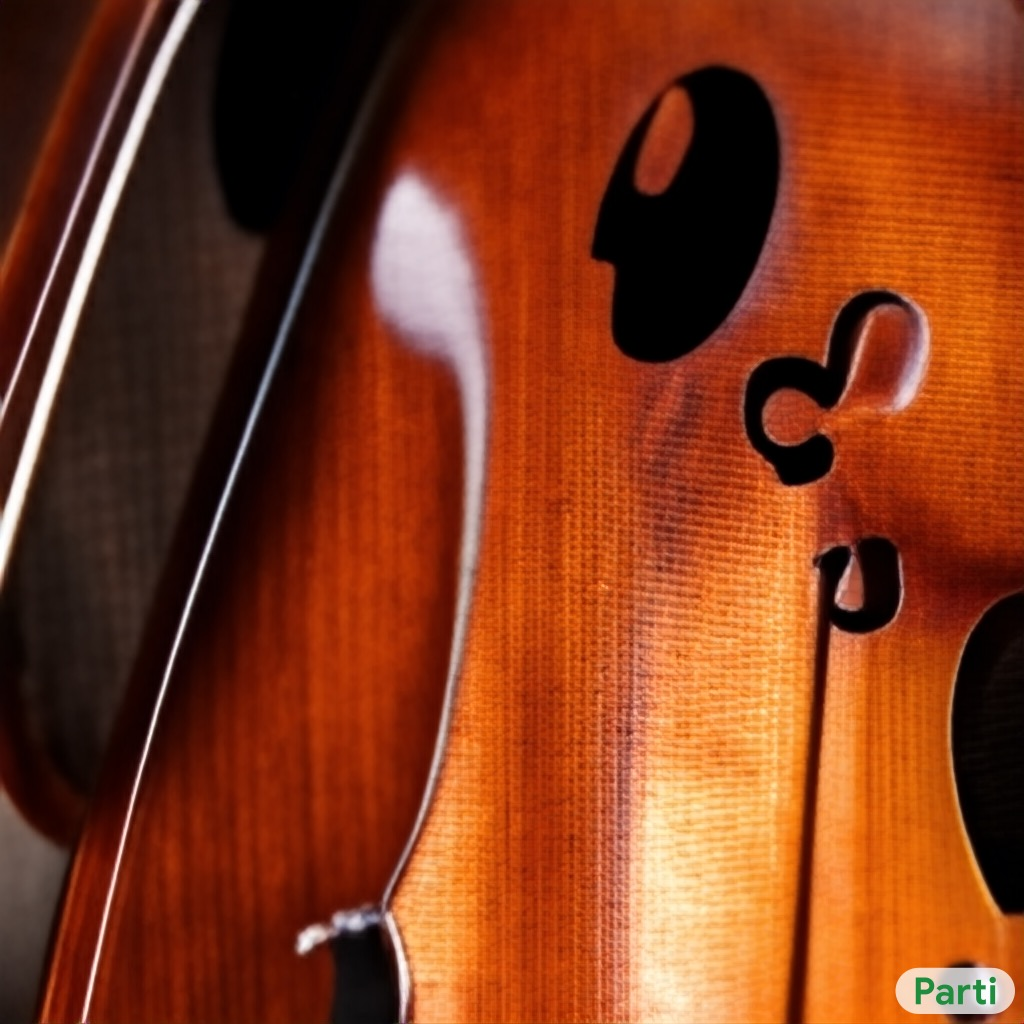
\includegraphics[width=0.24\textwidth]{figures/scaling_comparison/violin_1.jpg} &
        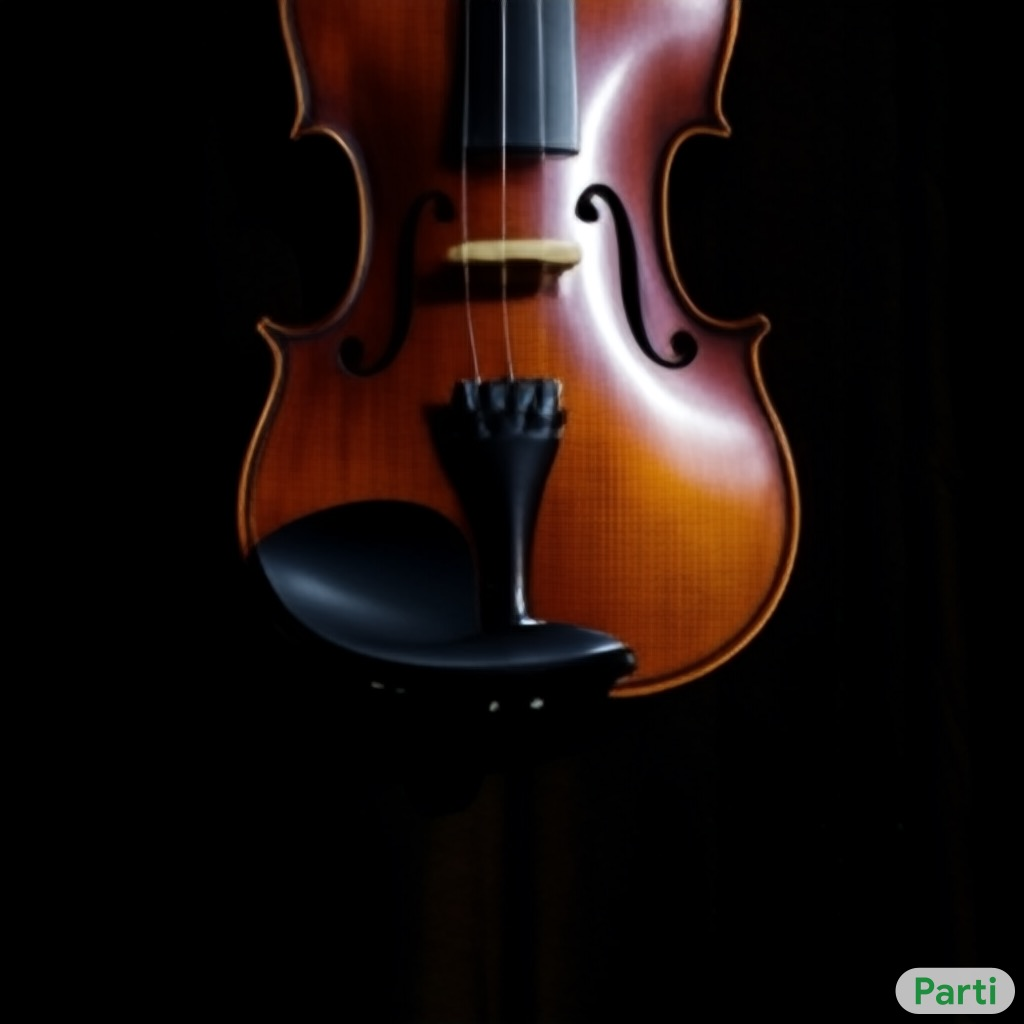
\includegraphics[width=0.24\textwidth]{figures/scaling_comparison/violin_2.jpg} &
        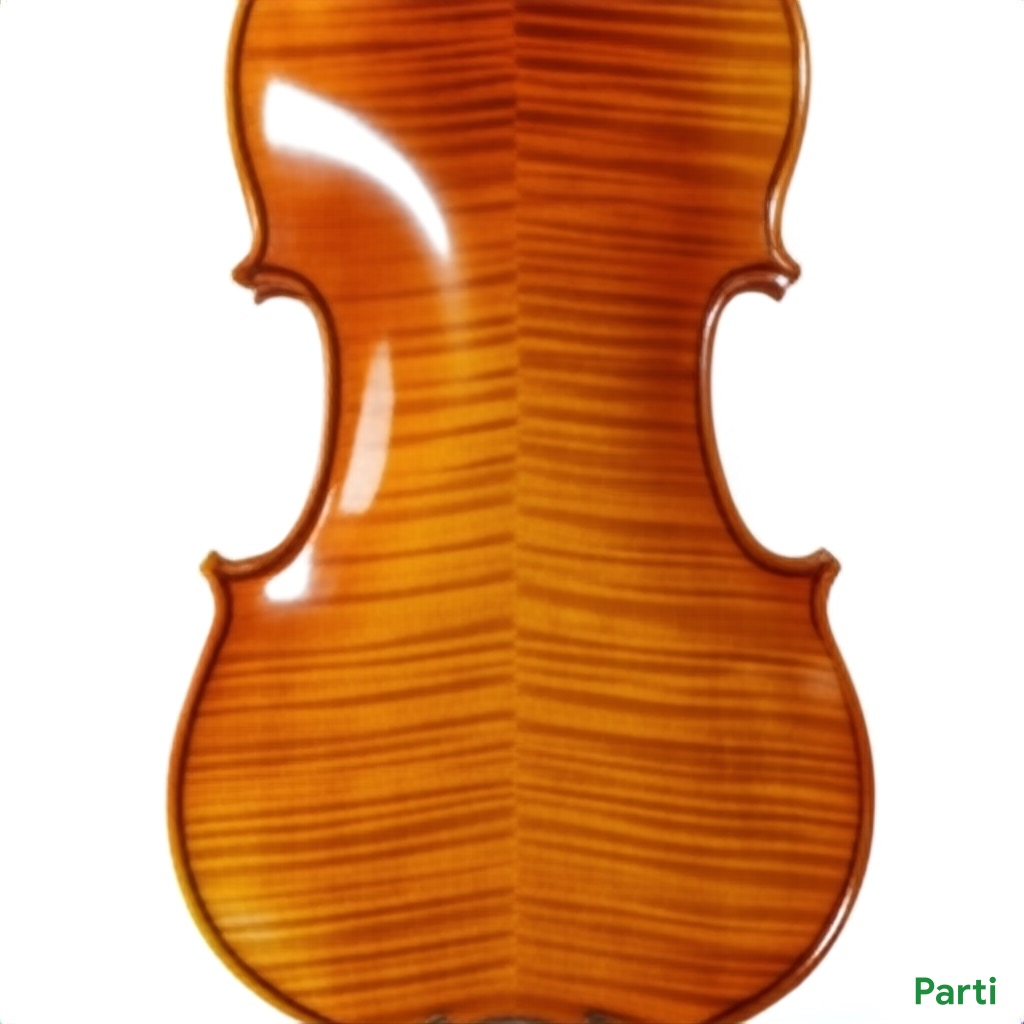
\includegraphics[width=0.24\textwidth]{figures/scaling_comparison/violin_3.jpg}\vspace{1mm} \\
        \multicolumn{4}{c}{\small The back of a violin}\vspace{3mm}\\

        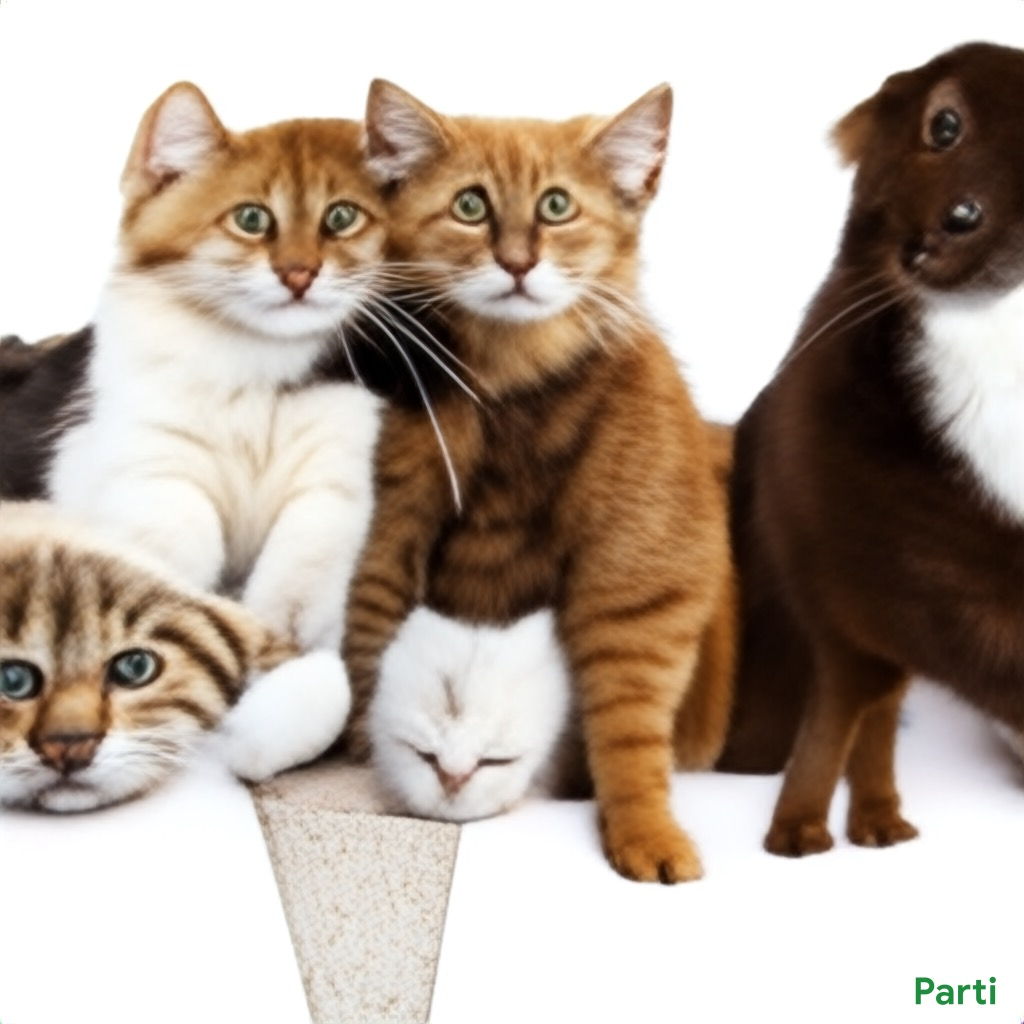
\includegraphics[width=0.24\textwidth]{figures/scaling_comparison/surrounding_0.jpg} &
        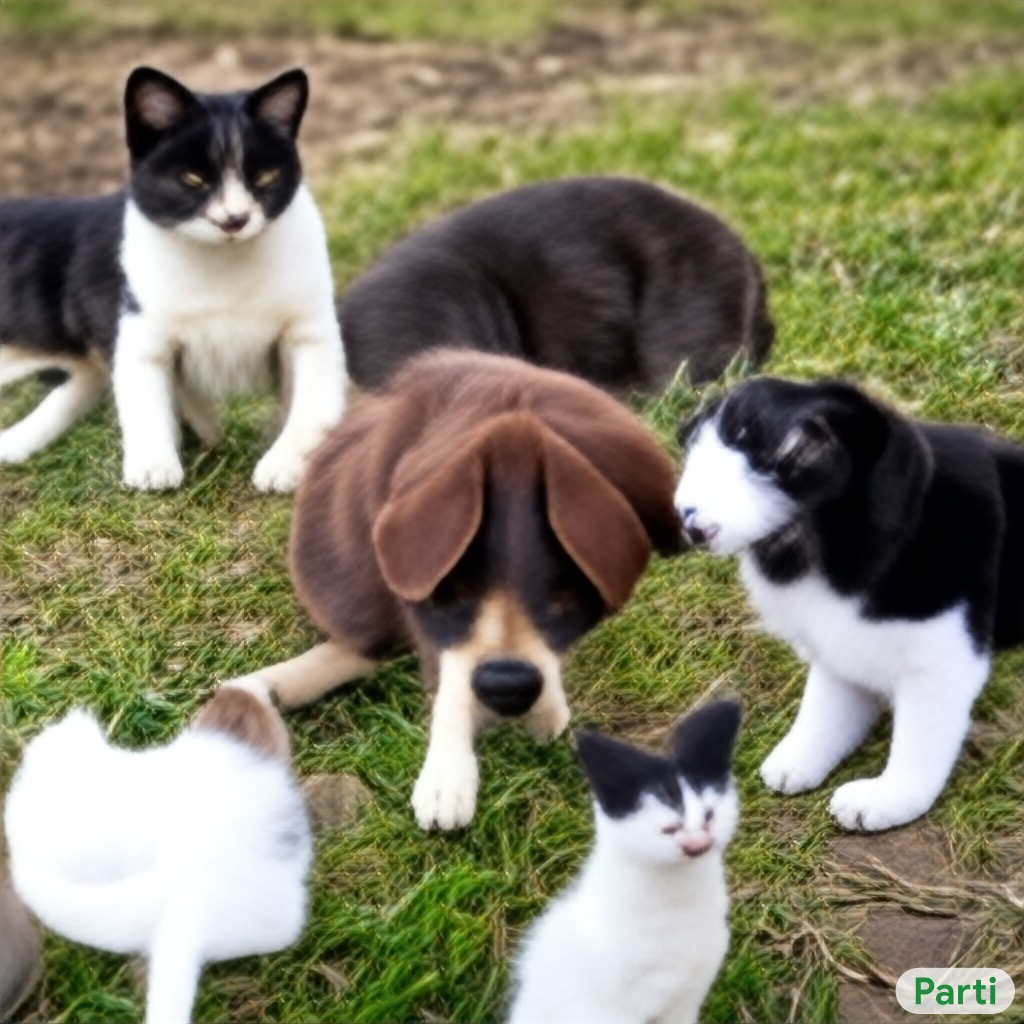
\includegraphics[width=0.24\textwidth]{figures/scaling_comparison/surrounding_1.jpg} &
        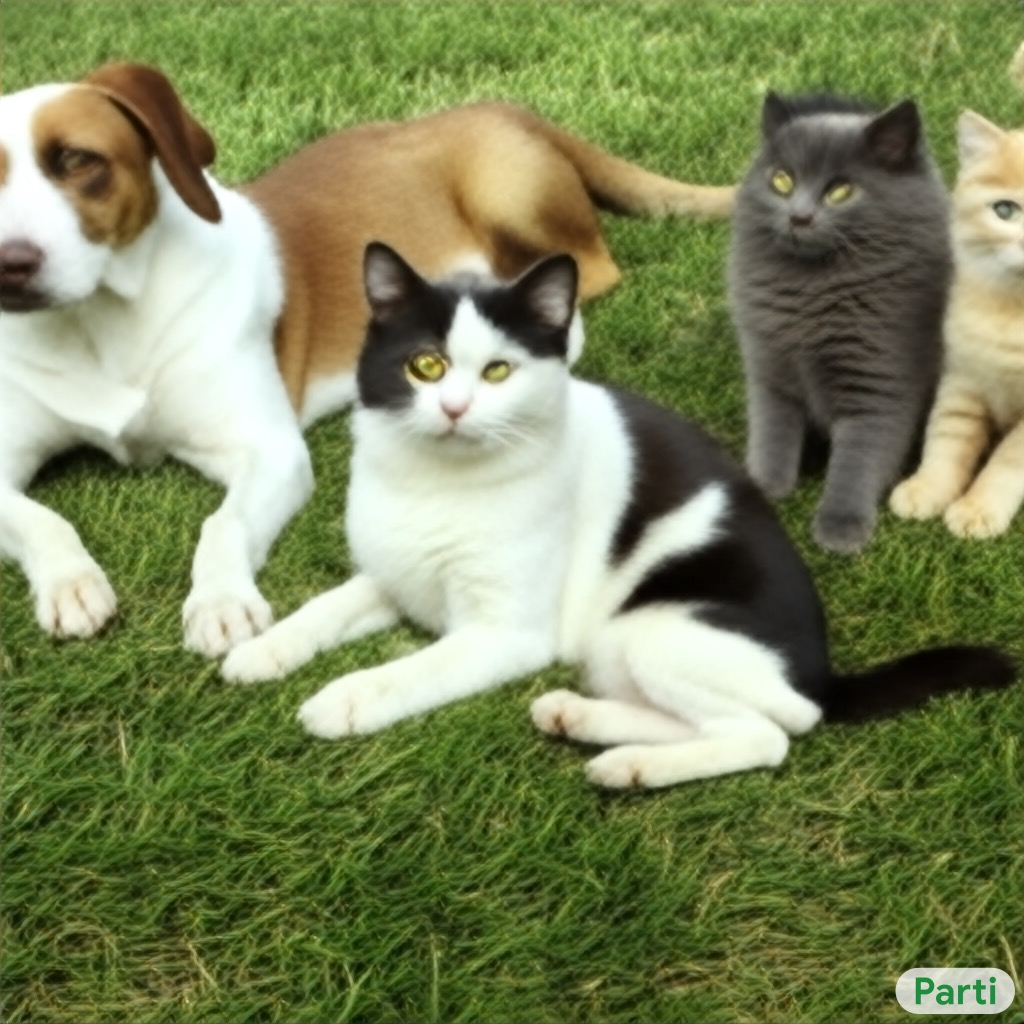
\includegraphics[width=0.24\textwidth]{figures/scaling_comparison/surrounding_2.jpg} &
        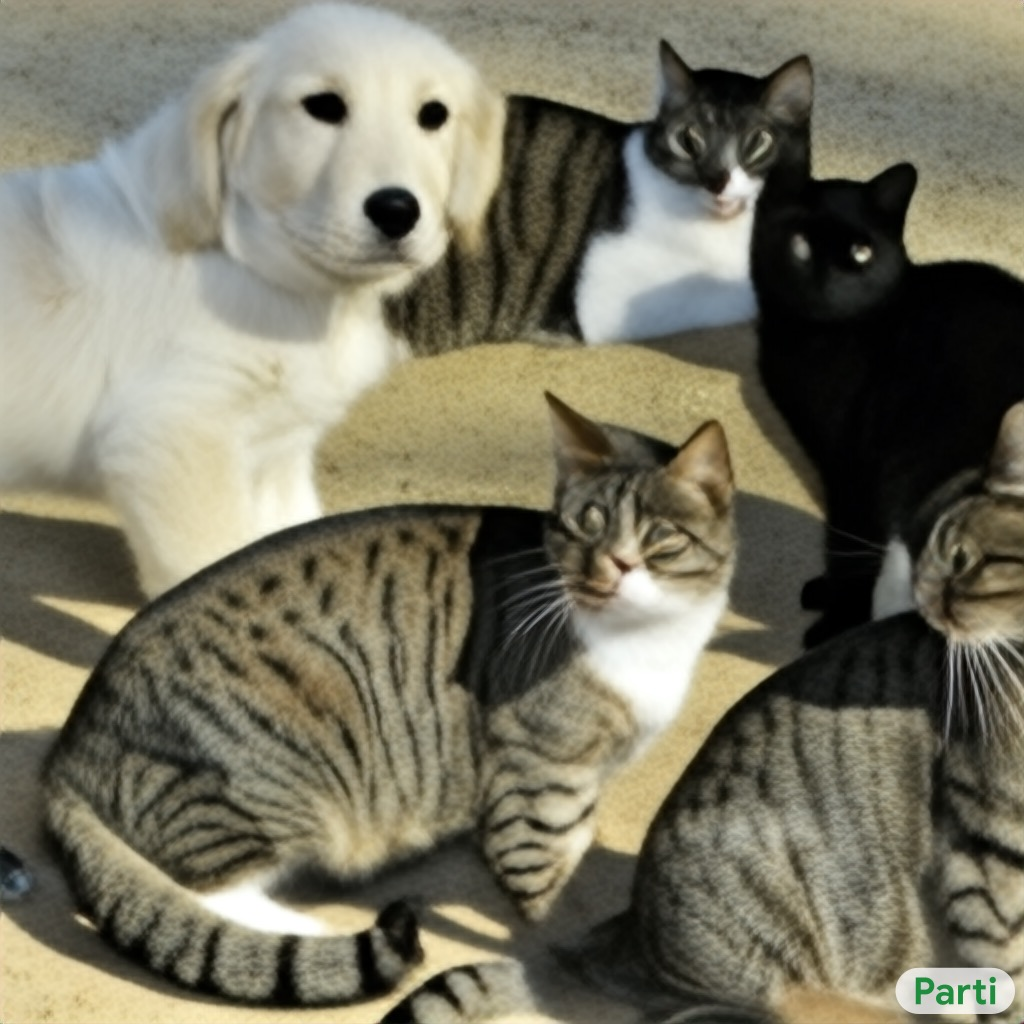
\includegraphics[width=0.24\textwidth]{figures/scaling_comparison/surrounding_3.jpg}\vspace{1mm} \\
        \multicolumn{4}{c}{\small Four cats surrounding a dog}\vspace{3mm}\\

        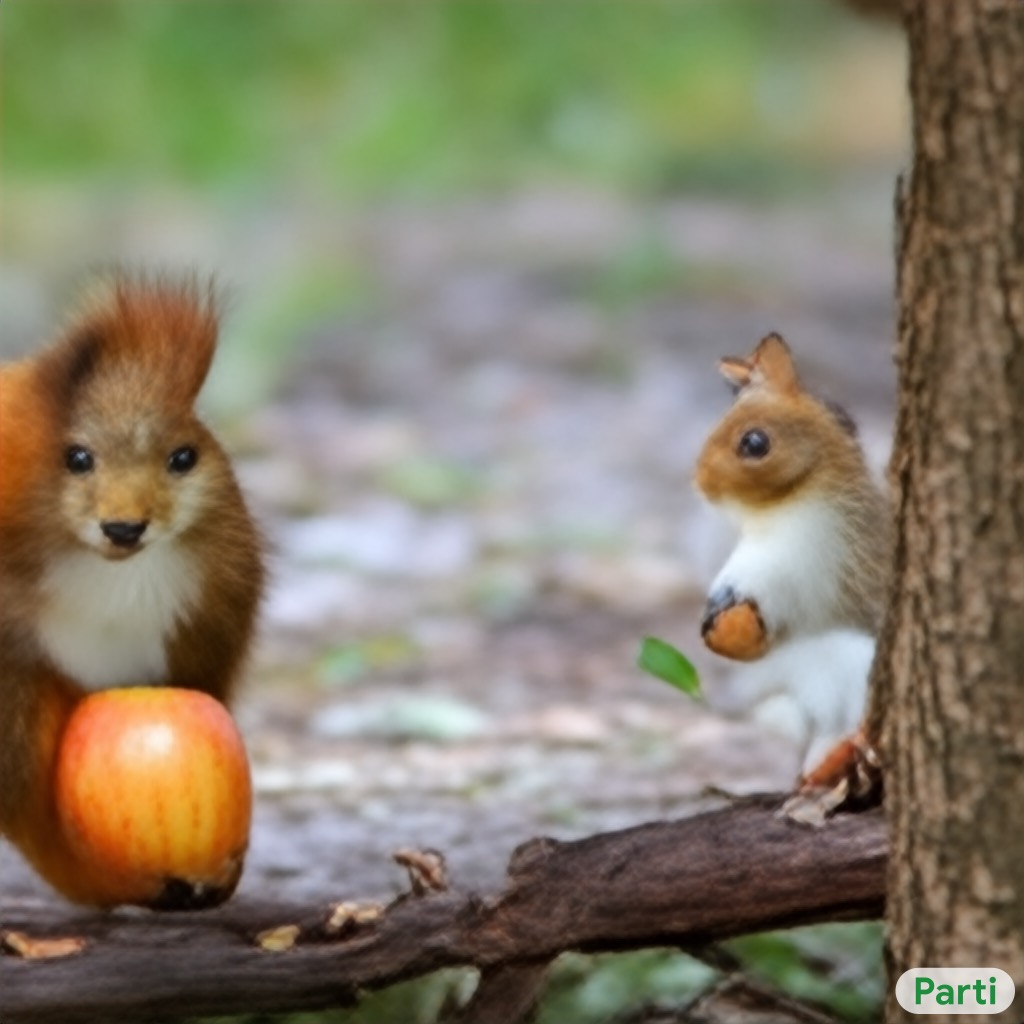
\includegraphics[width=0.24\textwidth]{figures/scaling_comparison/apple_0.jpg} &
        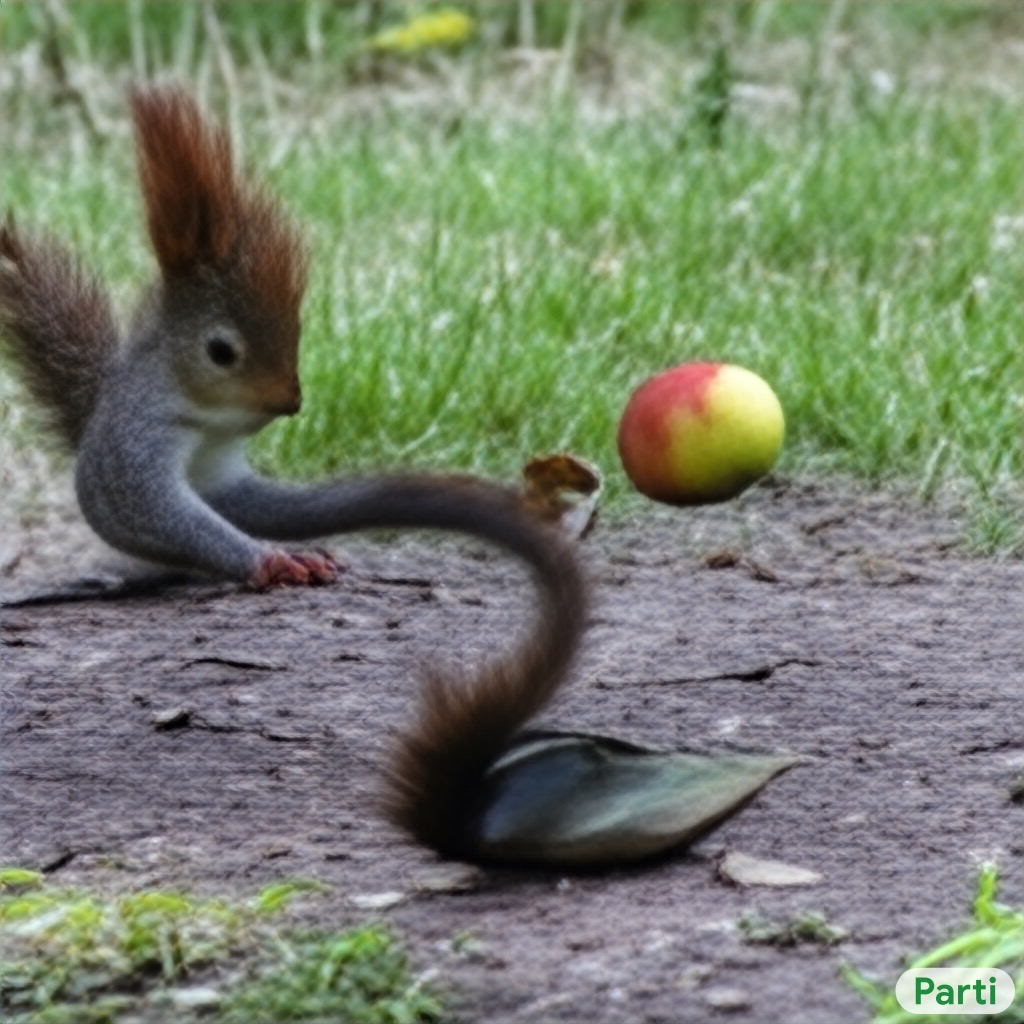
\includegraphics[width=0.24\textwidth]{figures/scaling_comparison/apple_1.jpg} &
        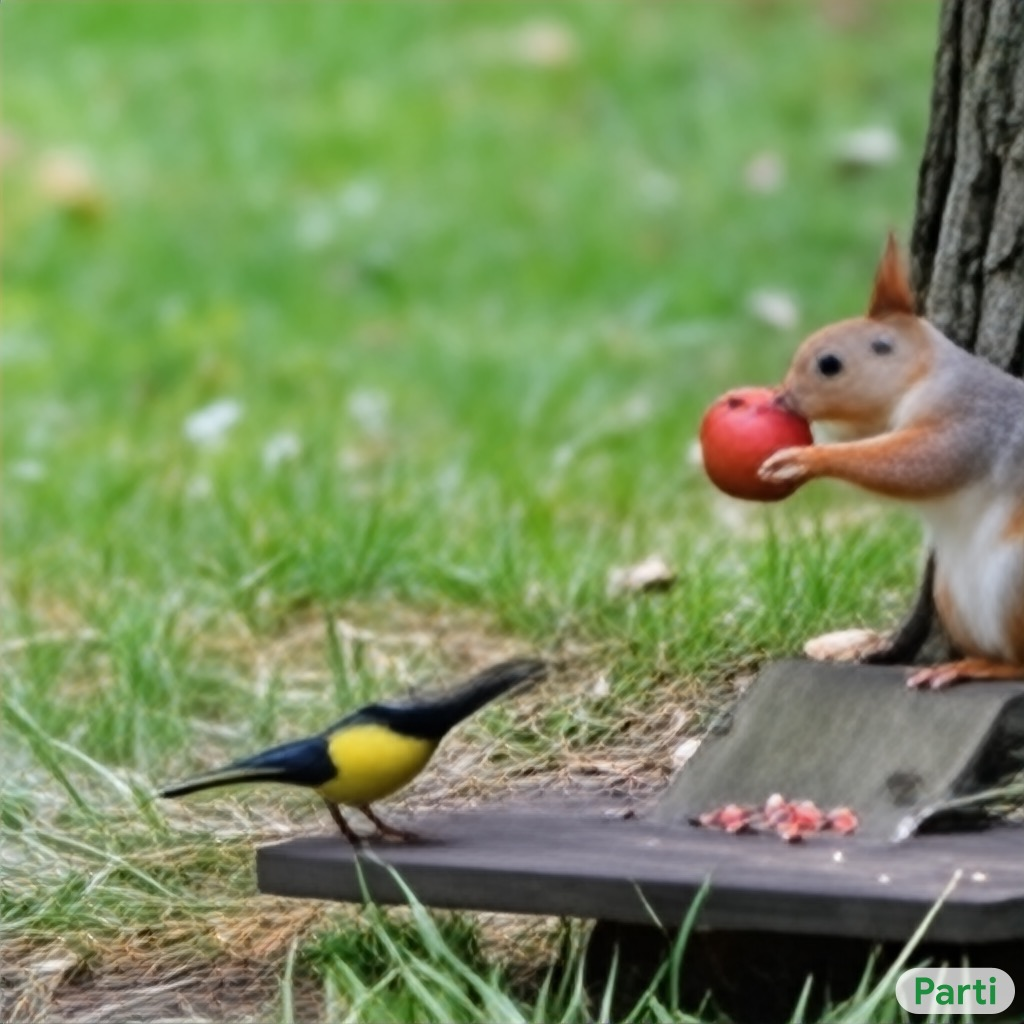
\includegraphics[width=0.24\textwidth]{figures/scaling_comparison/apple_2.jpg} &
        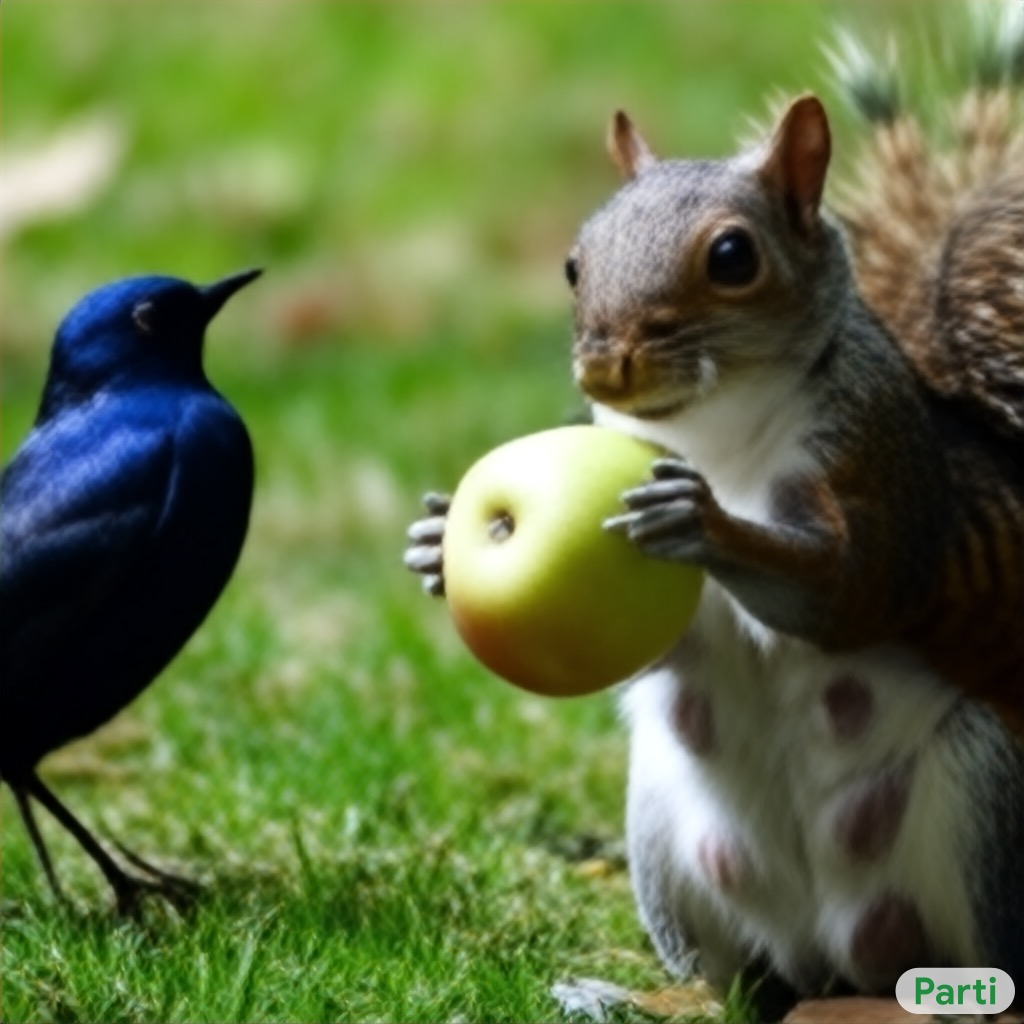
\includegraphics[width=0.24\textwidth]{figures/scaling_comparison/apple_3.jpg}\vspace{1mm} \\
        \multicolumn{4}{c}{\small A squirrel gives an apple to a bird}\vspace{3mm}\\

        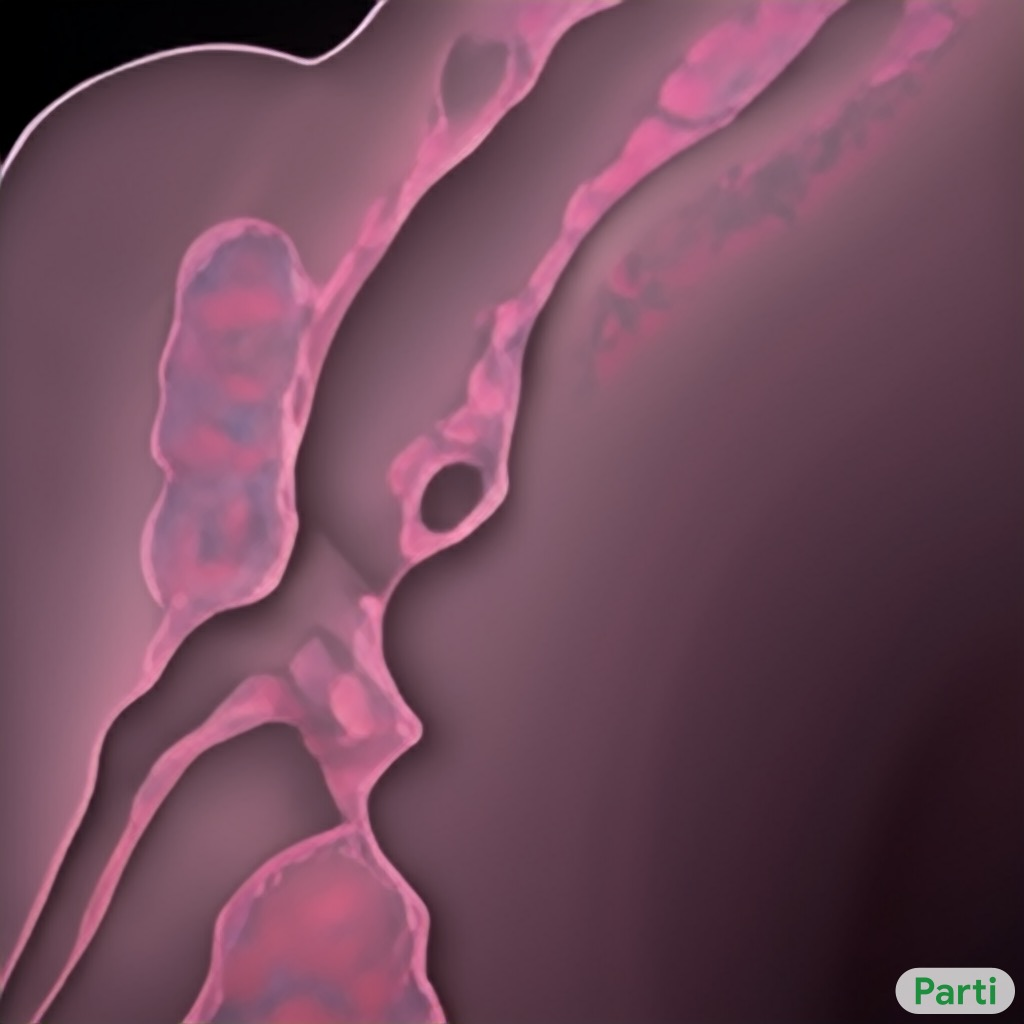
\includegraphics[width=0.24\textwidth]{figures/scaling_comparison/med_0.jpg} &
        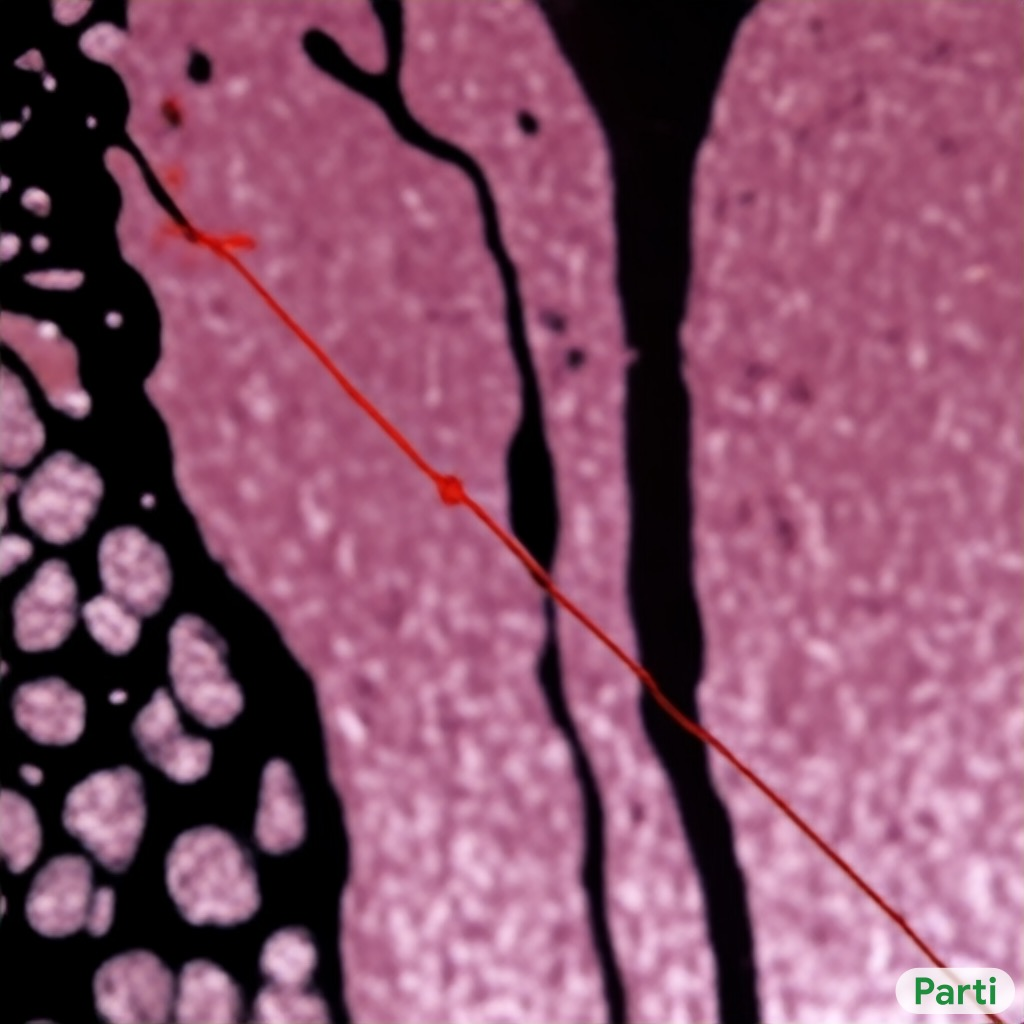
\includegraphics[width=0.24\textwidth]{figures/scaling_comparison/med_1.jpg} &
        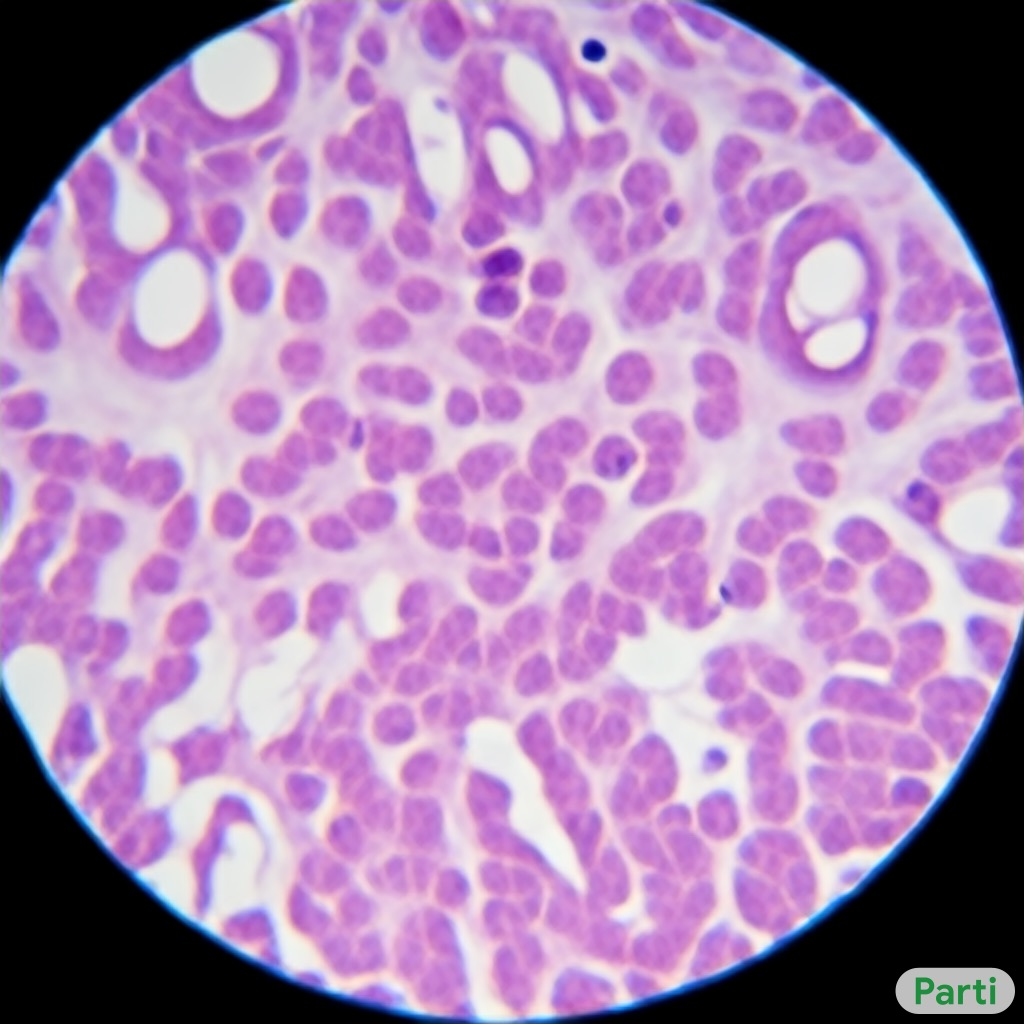
\includegraphics[width=0.24\textwidth]{figures/scaling_comparison/med_2.jpg} &
        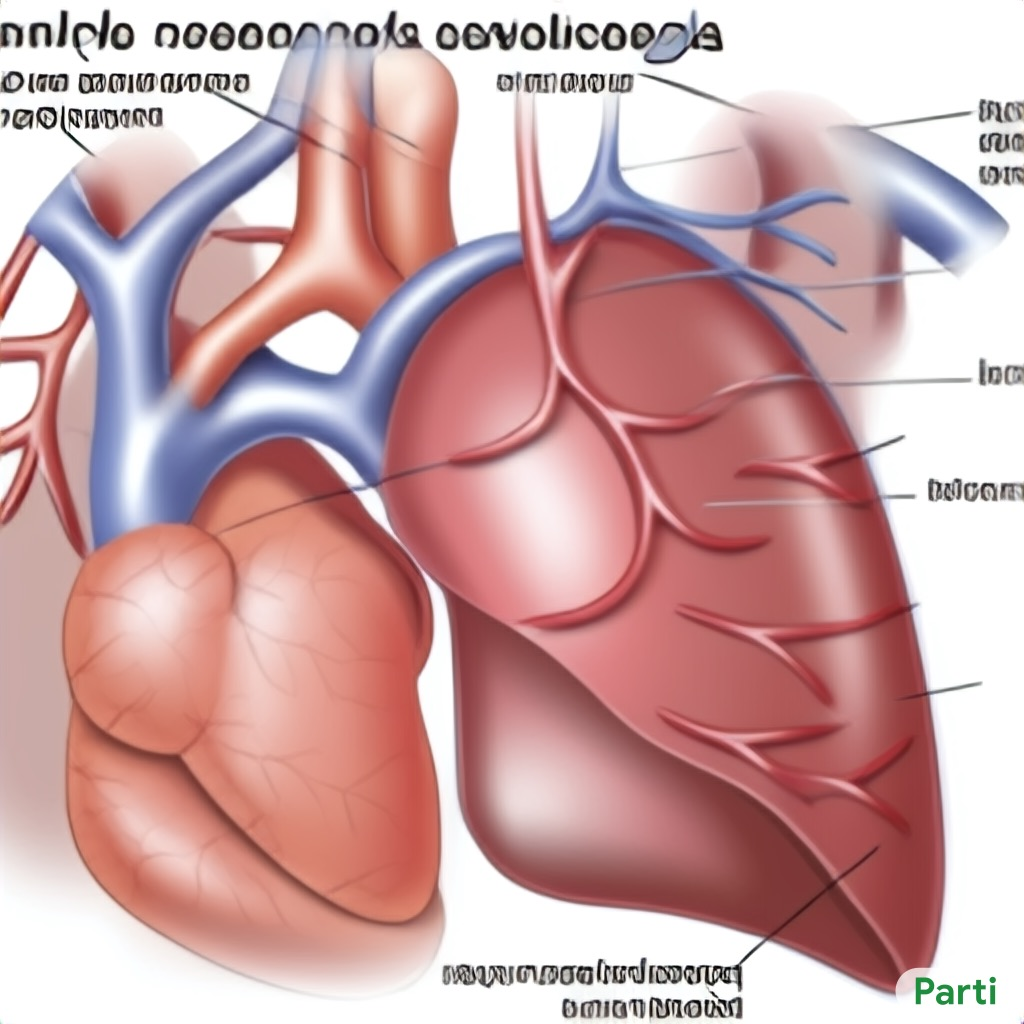
\includegraphics[width=0.24\textwidth]{figures/scaling_comparison/med_3.jpg}\vspace{1mm} \\
        \multicolumn{4}{c}{\small Pneumonoultramicroscopicsilicovolcanoconiosis} \\
    \end{tabular} 
    \caption{Qualitative comparison of scaling \bdraw models, similar to Figure~\ref{figs:scaling_comparison}. We show that simple prompts from the \bcpa{} benchmark (Section~\ref{secs:bcp}) can also be quite challenging. These examples test concepts such as \bcpstyle{Abstract}, \bcpstyle{Perspective}, \bcpstyle{Quantity}, and \bcpstyle{Linguistic Structure}.}
    \vspace{-0.15in}
    \label{figs:scaling_bcp}
\end{figure}

To better understand the improvements of the 20B over the 3B models, Figure~\ref{figs:bcp_20b_3b_language} further breaks down human preferences of the 20B model in terms of \textit{image-text match} across \bcpa{} categories (left) and challenge aspects (right). In terms of categories, the 20B model is clearly preferred over most categories, especially \bcpstyle{Abstract}, \bcpstyle{World Knowledge}, \bcpstyle{Vehicles}, and \bcpstyle{Arts}. The 20B and 3B models are on par for \bcpstyle{Produce \& Plants}.
In terms of challenge aspects, the 20B model are better over all dimensions, especially \bcpstyle{Writing \& Symbols}, \bcpstyle{Perspective}, and \bcpstyle{Imagination}. See Appendix~\ref{secs:appendix_bcp_evals} for full breakdown on image realism and image-text match for both the Retrieval baseline and the 3B model.



\textbf{Qualitative comparison.}
To understand qualitatively the effect of scaling, we present in Figure~\ref{figs:scaling_comparison} and \ref{figs:scaling_bcp} non-cherry-picked top-1 images sampled from \bdraw models of increasing sizes (350M, 750M, 3B, 20B). All model variants use the same image tokenizer and CoCa reranking model, described in Section~\ref{secs:sampling_cf_coca}, with sampling of 16 images per text prompt. We use prompts from the \bcpa{} benchmark to test the models' capabilities across a range of categories and challenging aspects.

Figure~\ref{figs:scaling_comparison} clearly shows improved quality as we scale up model size. The 3B model is, sometimes, as good as the 20B one in terms of the visual quality and image-text alignment for \bcpstyle{Fine-grained Detail} prompts such as ``astronaut riding a horse'' with ``water lilies''. The ``blue Porsche 356'' over ``yellow brick wall'' is a strong test of world knowledge: only the 20B model gets it right. The 3B model produces a visually clean car, but it is one which never existed -- it seems to merge features of multiple two-seater sports cars from the 1960s. When it comes to more challenging prompts such as those that test \bcpstyle{World Knowledge} and \bcpstyle{Writing \& Symbols}, the 20B model is able to produce better compositions, such as the ``kangaroo wearing an orange hoodie and blue sunglasses'' over the ``Sydney Opera House'' and the sushi-made ``map of United States'' (interestingly with wasabi in the map from the 20B model), as well as precise text outputs, such as ``Welcome Friends!'' and ``Very Deep Learning'', compared to those of the 3B model.

Figure~\ref{figs:scaling_bcp} examines models from a different perspective by demonstrating that short prompts in the \bcpa{} can also be quite challenging. The 20B model shows its strong visual abilities when generating \bcpstyle{Abstract} concepts, \eg, the ``infinity'' sign, and atypical \bcpstyle{Perspective}, \eg, ``the back of a violin.'' While both the 3B and 20B models generate animals rather well, the 20B model shines with more photorealistic outputs, \eg, for the prompt ``a squirrel gives an apple to a bird'', and correct \bcpstyle{Quantity} in the case of ``Four cats surrounding a dog''. Lastly, for the \bcpstyle{Linguistic Structure} example of ``Pneumonoultramicroscopicsilicovolcanoconiosis'', considered to be the longest English word (related to a lung disease), the 20B model generates a reasonable illustration of a lung.